\documentclass{ieeeaccess}
% IEEE Access version. The body, appendix, data statement and acknowledgment are shared with the
% arXiv version (main.tex) through body.tex and back.tex; every number is a macro generated by
% scripts/10_generate_macros.py. Build with: python scripts/build_submissions.py
\usepackage{cite}
\usepackage{amsmath,amssymb}
\usepackage{graphicx}
\usepackage{booktabs}
\usepackage{array}
\usepackage{url}
\def\UrlBreaks{\do\/\do-}

% Auto-generated by scripts/10_generate_macros.py -- DO NOT EDIT.
% Every number quoted in paper/main.tex is defined here.
\newcommand{\AlertsPerDefectMax}{154}
\newcommand{\AlertsPerDefectMin}{138}
\newcommand{\BOneBTwoHoursDiffMax}{3}
\newcommand{\BenchBank}{13{,}798}
\newcommand{\BenchCategory}{hazelnut}
\newcommand{\BenchFitImages}{313}
\newcommand{\BenchFps}{30}
\newcommand{\BenchFrames}{110}
\newcommand{\BenchRepeats}{5}
\newcommand{\BenchWindow}{30}
\newcommand{\BudgetFeasible}{5}
\newcommand{\BudgetFprMedian}{0.48}
\newcommand{\CorrMcProbLMax}{59}
\newcommand{\CorrMcProbLMin}{52}
\newcommand{\CorrRecallLossFull}{2.6}
\newcommand{\CorrReviewersBThreeMax}{5}
\newcommand{\CorrReviewersBThreeMin}{4}
\newcommand{\CorrReviewersETwoMax}{5}
\newcommand{\CorrReviewersETwoMin}{3}
\newcommand{\CorrRhoBThreeMax}{4.6}
\newcommand{\CorrRhoBThreeMin}{3.5}
\newcommand{\CounterIdleMaxW}{110}
\newcommand{\CounterIdleMinW}{77}
\newcommand{\CrHiresActiveW}{5.23}
\newcommand{\CrHiresEnergyRatio}{6.2}
\newcommand{\CrHiresFrameMJ}{174}
\newcommand{\CrHiresMvtecRecall}{0.95}
\newcommand{\CrHiresPaybackMin}{283}
\newcommand{\CrHiresRecall}{0.89}
\newcommand{\CrHiresVisaRecall}{0.72}
\newcommand{\CrHiresWorstRecall}{0.42}
\newcommand{\CrPcActiveW}{0.85}
\newcommand{\CrPcFrameMJ}{28}
\newcommand{\CrPcMvtecRecall}{0.94}
\newcommand{\CrPcRecall}{0.79}
\newcommand{\CrPcVisaRecall}{0.57}
\newcommand{\CrPcWorstRecall}{0.14}
\newcommand{\CrPdActiveW}{1.96}
\newcommand{\CrPdFrameMJ}{65}
\newcommand{\CrPdMvtecRecall}{0.63}
\newcommand{\CrPdRecall}{0.42}
\newcommand{\CrPdVisaRecall}{0.16}
\newcommand{\CrPdWorstRecall}{0.01}
\newcommand{\CrWrnActiveW}{3.13}
\newcommand{\CrWrnEnergyRatio}{3.7}
\newcommand{\CrWrnFrameMJ}{104}
\newcommand{\CrWrnMvtecRecall}{0.98}
\newcommand{\CrWrnRecall}{0.83}
\newcommand{\CrWrnVisaRecall}{0.55}
\newcommand{\CrWrnWorstRecall}{0.02}
\newcommand{\CudaRuntime}{12.1}
\newcommand{\DetAboveManualStar}{7}
\newcommand{\DetAurocMax}{1.000}
\newcommand{\DetAurocMin}{0.717}
\newcommand{\DetBankMax}{42{,}571}
\newcommand{\DetBankMin}{2{,}822}
\newcommand{\DetCategories}{27}
\newcommand{\DetFprMax}{26.4}
\newcommand{\DetFprMin}{0.8}
\newcommand{\DetGoodEvalMin}{24}
\newcommand{\DetMvtecCategories}{15}
\newcommand{\DetPcBeatsPdAuroc}{25}
\newcommand{\DetPcMvtecAurocMedian}{0.988}
\newcommand{\DetPcMvtecRecallMedian}{0.94}
\newcommand{\DetPcVisaAurocMedian}{0.939}
\newcommand{\DetPcVisaRecallMedian}{0.57}
\newcommand{\DetPdMvtecAurocMedian}{0.922}
\newcommand{\DetPdMvtecRecallMedian}{0.63}
\newcommand{\DetPdVisaAurocMedian}{0.874}
\newcommand{\DetPdVisaRecallMedian}{0.16}
\newcommand{\DetRecallMax}{1.00}
\newcommand{\DetRecallMedian}{0.792}
\newcommand{\DetRecallMin}{0.14}
\newcommand{\DetSeedList}{0, 1, 2}
\newcommand{\DetSeeds}{3}
\newcommand{\DetVisaCategories}{12}
\newcommand{\DetWorstCategory}{macaroni2}
\newcommand{\EOneLateGapMax}{1}
\newcommand{\EOneRecallLoss}{4.2}
\newcommand{\EdgeBenefitRatioMax}{5{,}200}
\newcommand{\EdgeBenefitRatioMin}{72}
\newcommand{\EdgeOfBenefitMax}{1.4}
\newcommand{\EdgePrccMax}{0.02}
\newcommand{\EdgeShareMax}{0.51}
\newcommand{\EdgeSobolMax}{\ensuremath{9\times10^{-6}}}
\newcommand{\EscapeShareMax}{35}
\newcommand{\EscapeShareMin}{24}
\newcommand{\FrameEnergyRatio}{10}
\newcommand{\FullActivePower}{8.46}
\newcommand{\FullActivePowerMax}{9.01}
\newcommand{\FullActivePowerMin}{7.15}
\newcommand{\FullFrameEnergy}{0.282}
\newcommand{\FullFrameEnergyMax}{0.301}
\newcommand{\FullFrameEnergyMin}{0.239}
\newcommand{\FullLatencyMs}{14.8}
\newcommand{\FullMaxFps}{141}
\newcommand{\FullTotalPower}{10.34}
\newcommand{\GpuDriver}{581.86}
\newcommand{\GpuName}{RTX 4050 Laptop GPU}
\newcommand{\HiValBOneCarbonEdge}{4}
\newcommand{\HiValCarbonBThree}{8{,}284}
\newcommand{\HiValCarbonBZero}{8{,}330}
\newcommand{\HiValCarbonLZero}{10{,}425}
\newcommand{\HiValCellHeadroom}{16{,}636}
\newcommand{\HiValCellPowerStar}{265}
\newcommand{\HiValCorrDeltaCETwo}{2{,}148}
\newcommand{\HiValCorrDeltaCvsLZero}{1{,}889}
\newcommand{\HiValCorrMcProb}{51.6}
\newcommand{\HiValCorrOmegaStar}{0.20}
\newcommand{\HiValCorrPpvBThree}{0.9}
\newcommand{\HiValCrHiresExtra}{0.036}
\newcommand{\HiValCrHiresGain}{1{,}162}
\newcommand{\HiValCrHiresShare}{89}
\newcommand{\HiValCrPcShare}{59}
\newcommand{\HiValCrPdShare}{33}
\newcommand{\HiValCrWrnShare}{67}
\newcommand{\HiValDelayMaterialCost}{0.503}
\newcommand{\HiValDeltaCBZerovsLZero}{2{,}095}
\newcommand{\HiValDeltaCEOne}{1{,}732}
\newcommand{\HiValDeltaCvsBOne}{-4.01}
\newcommand{\HiValDeltaCvsBTwo}{4.9}
\newcommand{\HiValDeltaCvsBZero}{46.1}
\newcommand{\HiValDeltaCvsLZero}{2{,}141}
\newcommand{\HiValDeltaCvsNZero}{9{,}794}
\newcommand{\HiValDeltaEvsBZero}{233}
\newcommand{\HiValDeltaEvsLZero}{-93.8}
\newcommand{\HiValDeltaHvsBZero}{2{,}736}
\newcommand{\HiValDeltaHvsLZero}{-3.75}
\newcommand{\HiValDeltaMvsLZero}{79.4}
\newcommand{\HiValEdgeCarbon}{0.409}
\newcommand{\HiValEdgeKWh}{0.532}
\newcommand{\HiValEdgeOfBenefit}{0.019}
\newcommand{\HiValEdgeShare}{0.0049}
\newcommand{\HiValEscapeShare}{35}
\newcommand{\HiValHoursBThree}{12.1}
\newcommand{\HiValHoursBZero}{2{,}748}
\newcommand{\HiValHoursLZero}{8.33}
\newcommand{\HiValManualRecallStar}{0.96}
\newcommand{\HiValMcEdgeShareHigh}{0.0099}
\newcommand{\HiValMcHigh}{4{,}995}
\newcommand{\HiValMcLow}{-6{,}832}
\newcommand{\HiValMcMedian}{317}
\newcommand{\HiValMcProb}{53.7}
\newcommand{\HiValMcProbBThree}{53.7}
\newcommand{\HiValMcProbBZero}{45}
\newcommand{\HiValMcProbNZero}{100.0}
\newcommand{\HiValOmegaStar}{0.24}
\newcommand{\HiValOptRhoMax}{0.3}
\newcommand{\HiValOptSavingCapMax}{8{,}501}
\newcommand{\HiValOptSavingCapShare}{100}
\newcommand{\HiValOptSavingMax}{8{,}501}
\newcommand{\HiValPiStarLZero}{17}
\newcommand{\HiValPiStarNZero}{5}
\newcommand{\HiValPpvBThree}{8}
\newcommand{\HiValPpvEOne}{26}
\newcommand{\HiValRecallLossStar}{0.471}
\newcommand{\HiValRelCarbonReduction}{21}
\newcommand{\HiValReviewersBOne}{8}
\newcommand{\HiValReviewersBThree}{1}
\newcommand{\HiValReviewersBZero}{83}
\newcommand{\HiValRhoBOne}{7.34}
\newcommand{\HiValRhoBThree}{0.36}
\newcommand{\HiValRhoBTwo}{7.51}
\newcommand{\HiValRhoBZero}{82.43}
\newcommand{\HiValRhoLZero}{0.25}
\newcommand{\HiValSE}{-0.99}
\newcommand{\HiValSH}{-0.31}
\newcommand{\HiValSobolTop}{detector recall}
\newcommand{\HiValSobolTopST}{0.96}
\newcommand{\HiValSqiBal}{-0.21}
\newcommand{\HiValSqiRobust}{18}
\newcommand{\HiValTfu}{33.3}
\newcommand{\HiValTopPrcc}{+0.97}
\newcommand{\HiValVisaDeltaCvsLZero}{-108}
\newcommand{\HiValVisaETwoDeltaC}{1{,}300}
\newcommand{\HiValVisibleFrames}{15}
\newcommand{\HiValVisibleMs}{500}
\newcommand{\HostPowerCentral}{12}
\newcommand{\HwDoubledEdgeOfBenefitMax}{2.4}
\newcommand{\HwStarMultLZeroMin}{105}
\newcommand{\HwStarMultNZeroMin}{304}
\newcommand{\IdlePower}{1.88}
\newcommand{\IdleReadingsMin}{50}
\newcommand{\InferActivePower}{8.49}
\newcommand{\InferFrameEnergy}{0.283}
\newcommand{\InferLatencyMs}{14.9}
\newcommand{\InferMaxFps}{163}
\newcommand{\InferTotalPower}{10.58}
\newcommand{\JetsonCellPower}{16}
\newcommand{\JetsonComputeShare}{25}
\newcommand{\JetsonFullActivePower}{0.85}
\newcommand{\JetsonFullTotalPower}{3.98}
\newcommand{\JetsonIdlePower}{3.11}
\newcommand{\JetsonKernel}{6.8.12-1021-tegra}
\newcommand{\JetsonLft}{R39}
\newcommand{\JetsonModel}{Jetson Orin Nano}
\newcommand{\JetsonPcFullFrameMJ}{83}
\newcommand{\JetsonPcFullMaxFps}{86}
\newcommand{\JetsonPcFullMaxRelErr}{0.038}
\newcommand{\JetsonPcFullTotalPower}{5.8}
\newcommand{\JetsonPcHalfFrameMJ}{28}
\newcommand{\JetsonPcHalfMaxFps}{243}
\newcommand{\JetsonPcHalfMaxRelErr}{0.8}
\newcommand{\JetsonPcHalfTotalPower}{4.0}
\newcommand{\JetsonPdFullFrameMJ}{84}
\newcommand{\JetsonPdFullMaxFps}{81}
\newcommand{\JetsonPdFullMaxRelErr}{0.34}
\newcommand{\JetsonPdFullTotalPower}{5.6}
\newcommand{\JetsonPdHalfFrameMJ}{65}
\newcommand{\JetsonPdHalfMaxFps}{107}
\newcommand{\JetsonPdHalfMaxRelErr}{0.48}
\newcommand{\JetsonPdHalfTotalPower}{5.1}
\newcommand{\JetsonPowerMode}{15W}
\newcommand{\JetsonPython}{3.12.3}
\newcommand{\JetsonTensorRT}{10.16}
\newcommand{\ManualRecallCentral}{0.75}
\newcommand{\McProbLMax}{64}
\newcommand{\McProbLMin}{54}
\newcommand{\MetalCarbonBThree}{128}
\newcommand{\MetalCarbonBZero}{142}
\newcommand{\MetalCarbonLZero}{175}
\newcommand{\MetalCellHeadroom}{1{,}484}
\newcommand{\MetalCellPowerStar}{23.7}
\newcommand{\MetalCorrDeltaCETwo}{47.5}
\newcommand{\MetalCorrDeltaCvsLZero}{41.2}
\newcommand{\MetalCorrMcProb}{51.8}
\newcommand{\MetalCorrOmegaStar}{0.18}
\newcommand{\MetalCorrPpvBThree}{1.4}
\newcommand{\MetalCrHiresExtra}{0.0089}
\newcommand{\MetalCrHiresGain}{27.9}
\newcommand{\MetalCrHiresShare}{85}
\newcommand{\MetalCrPcShare}{59}
\newcommand{\MetalCrPdShare}{33}
\newcommand{\MetalCrWrnShare}{67}
\newcommand{\MetalDeltaCBZerovsLZero}{33.3}
\newcommand{\MetalDeltaCEOne}{38}
\newcommand{\MetalDeltaCvsBOne}{1.56}
\newcommand{\MetalDeltaCvsBTwo}{1.67}
\newcommand{\MetalDeltaCvsBZero}{14.4}
\newcommand{\MetalDeltaCvsLZero}{47.7}
\newcommand{\MetalDeltaCvsNZero}{235}
\newcommand{\MetalDeltaEvsBZero}{59.8}
\newcommand{\MetalDeltaEvsLZero}{-19.1}
\newcommand{\MetalDeltaHvsBZero}{703}
\newcommand{\MetalDeltaHvsLZero}{-0.386}
\newcommand{\MetalDeltaMvsLZero}{2.2}
\newcommand{\MetalEdgeCarbon}{0.102}
\newcommand{\MetalEdgeKWh}{0.133}
\newcommand{\MetalEdgeOfBenefit}{0.21}
\newcommand{\MetalEdgeShare}{0.08}
\newcommand{\MetalEscapeShare}{32}
\newcommand{\MetalHoursBThree}{3.16}
\newcommand{\MetalHoursBZero}{707}
\newcommand{\MetalHoursLZero}{2.78}
\newcommand{\MetalManualRecallStar}{0.94}
\newcommand{\MetalMcEdgeShareHigh}{0.21}
\newcommand{\MetalMcHigh}{90.1}
\newcommand{\MetalMcLow}{-120}
\newcommand{\MetalMcMedian}{6.2}
\newcommand{\MetalMcProb}{54.5}
\newcommand{\MetalMcProbBThree}{54.5}
\newcommand{\MetalMcProbBZero}{100}
\newcommand{\MetalMcProbNZero}{100.0}
\newcommand{\MetalOmegaStar}{0.23}
\newcommand{\MetalOptRhoMax}{1.2}
\newcommand{\MetalOptSavingCapMax}{200}
\newcommand{\MetalOptSavingCapShare}{99}
\newcommand{\MetalOptSavingMax}{204}
\newcommand{\MetalPiStarLZero}{64}
\newcommand{\MetalPiStarNZero}{20}
\newcommand{\MetalPpvBThree}{13}
\newcommand{\MetalPpvEOne}{36}
\newcommand{\MetalRecallLossStar}{6.11}
\newcommand{\MetalRelCarbonReduction}{27}
\newcommand{\MetalReviewersBThree}{1}
\newcommand{\MetalReviewersBZero}{85}
\newcommand{\MetalRhoBOne}{9.90}
\newcommand{\MetalRhoBThree}{0.38}
\newcommand{\MetalRhoBTwo}{10.15}
\newcommand{\MetalRhoBZero}{84.79}
\newcommand{\MetalRhoLZero}{0.33}
\newcommand{\MetalSE}{-0.86}
\newcommand{\MetalSH}{-0.12}
\newcommand{\MetalSobolTop}{detector recall}
\newcommand{\MetalSobolTopST}{0.97}
\newcommand{\MetalSqiBal}{-0.07}
\newcommand{\MetalSqiRobust}{42}
\newcommand{\MetalTfu}{8.33}
\newcommand{\MetalTopPrcc}{+0.96}
\newcommand{\MetalVisaDeltaCvsLZero}{-6.22}
\newcommand{\MetalVisaETwoDeltaC}{27.4}
\newcommand{\MetalVisibleFrames}{6}
\newcommand{\MetalVisibleMs}{200}
\newcommand{\MonteCarloDraws}{10{,}000}
\newcommand{\NomogramGramsPerHour}{28}
\newcommand{\OptCapRecallMedian}{0.99}
\newcommand{\OptFprMax}{57}
\newcommand{\OptFprMedian}{34.9}
\newcommand{\OptFprWorst}{53}
\newcommand{\OptMorePermissive}{74}
\newcommand{\OptPairs}{81}
\newcommand{\OptRecallWorstOpt}{0.82}
\newcommand{\OptRecallWorstQ}{0.14}
\newcommand{\OptWorstCategory}{macaroni2}
\newcommand{\OptWorstDataset}{VisA}
\newcommand{\PaperABank}{13{,}798}
\newcommand{\PaperACommit}{4752116}
\newcommand{\PaperACorrFaFull}{188.6}
\newcommand{\PaperADelay}{3.7}
\newcommand{\PaperAFaRaw}{4{,}616}
\newcommand{\PaperAGlareFull}{0.66}
\newcommand{\PaperAGlareRate}{30}
\newcommand{\PaperAGlareTimer}{0.03}
\newcommand{\PaperALoadCross}{40}
\newcommand{\PaperAMu}{60}
\newcommand{\PaperANumPolicies}{11}
\newcommand{\PaperAPerDefectFull}{1.00}
\newcommand{\PaperAPerDefectRaw}{137.64}
\newcommand{\PaperAShortK}{4}
\newcommand{\PaperAShortN}{10}
\newcommand{\PaperAShortRecallEight}{97}
\newcommand{\PaperAShortRecallOne}{10}
\newcommand{\PaperAVisaCategories}{12}
\newcommand{\PaperAVisaFaFull}{1.7}
\newcommand{\PaperAVisaPerDefectFull}{1.34}
\newcommand{\PaperAVisaRecallFull}{0.77}
\newcommand{\PaperAVisaRecallRaw}{0.99}
\newcommand{\PaperAVisionLatency}{16.9}
\newcommand{\PersistLossMax}{2.6}
\newcommand{\PlatformCarbonRatio}{1.9}
\newcommand{\PlatformDeltaCMax}{1.3}
\newcommand{\PolicyActivePower}{8.57}
\newcommand{\PolicyFrameEnergy}{0.286}
\newcommand{\PolicyLatencyMs}{14.7}
\newcommand{\PolicyMaxFps}{170}
\newcommand{\PolicyTotalPower}{10.56}
\newcommand{\PopEdgeShareAboveOne}{32}
\newcommand{\PopEdgeShareMedian}{0.19}
\newcommand{\PopEdgeShareNinetyFive}{35}
\newcommand{\PopHighShareBenefitMedian}{2.32}
\newcommand{\PopLowShareBenefitMedian}{129}
\newcommand{\PopSize}{20{,}000}
\newcommand{\PopWinLZero}{38.7}
\newcommand{\PopWinNZero}{85.6}
\newcommand{\PrecCarbonBThree}{1.35}
\newcommand{\PrecCarbonBZero}{3.94}
\newcommand{\PrecCarbonLZero}{1.83}
\newcommand{\PrecCellHeadroom}{229}
\newcommand{\PrecCellPowerStar}{3.65}
\newcommand{\PrecCorrDeltaCvsLZero}{0.415}
\newcommand{\PrecCorrMcProb}{58.9}
\newcommand{\PrecCorrOmegaStar}{0.39}
\newcommand{\PrecCorrPpvBThree}{25}
\newcommand{\PrecCrHiresExtra}{0.0006}
\newcommand{\PrecCrHiresGain}{0.169}
\newcommand{\PrecCrHiresShare}{96}
\newcommand{\PrecCrPcShare}{85}
\newcommand{\PrecCrPdShare}{33}
\newcommand{\PrecCrWrnShare}{81}
\newcommand{\PrecDeltaCBZerovsLZero}{-2.11}
\newcommand{\PrecDeltaCvsBOne}{1.88}
\newcommand{\PrecDeltaCvsBTwo}{1.94}
\newcommand{\PrecDeltaCvsBZero}{2.6}
\newcommand{\PrecDeltaCvsLZero}{0.488}
\newcommand{\PrecDeltaCvsNZero}{1.42}
\newcommand{\PrecDeltaEvsBZero}{10.7}
\newcommand{\PrecDeltaEvsLZero}{-1.02}
\newcommand{\PrecDeltaHvsBZero}{126}
\newcommand{\PrecDeltaHvsLZero}{-0.236}
\newcommand{\PrecDeltaMvsLZero}{0.162}
\newcommand{\PrecEdgeCarbon}{0.00682}
\newcommand{\PrecEdgeKWh}{0.00886}
\newcommand{\PrecEdgeOfBenefit}{1.4}
\newcommand{\PrecEdgeShare}{0.51}
\newcommand{\PrecEscapeShare}{24}
\newcommand{\PrecGammaStar}{0.72}
\newcommand{\PrecHoursBThree}{0.792}
\newcommand{\PrecHoursBZero}{127}
\newcommand{\PrecHoursLZero}{0.556}
\newcommand{\PrecManualRecallStar}{none}
\newcommand{\PrecMcEdgeShareHigh}{0.74}
\newcommand{\PrecMcHigh}{1.28}
\newcommand{\PrecMcLow}{-0.806}
\newcommand{\PrecMcMedian}{0.206}
\newcommand{\PrecMcProb}{64.3}
\newcommand{\PrecMcProbBThree}{64.3}
\newcommand{\PrecMcProbBZero}{100}
\newcommand{\PrecMcProbNZero}{100.0}
\newcommand{\PrecOmegaStar}{none}
\newcommand{\PrecOptRhoMax}{16.7}
\newcommand{\PrecOptSavingCapMax}{0.25}
\newcommand{\PrecOptSavingCapShare}{24}
\newcommand{\PrecOptSavingMax}{1.07}
\newcommand{\PrecPiStarLZero}{none}
\newcommand{\PrecPiStarNZero}{342}
\newcommand{\PrecPpvBThree}{77}
\newcommand{\PrecRecallLossStar}{none}
\newcommand{\PrecRelCarbonReduction}{27}
\newcommand{\PrecReviewersBThree}{2}
\newcommand{\PrecReviewersBZero}{229}
\newcommand{\PrecRhoBOne}{165.90}
\newcommand{\PrecRhoBThree}{1.43}
\newcommand{\PrecRhoBTwo}{171.09}
\newcommand{\PrecRhoBZero}{228.69}
\newcommand{\PrecRhoLZero}{1.00}
\newcommand{\PrecSE}{-0.84}
\newcommand{\PrecSH}{-0.30}
\newcommand{\PrecSobolTop}{detector recall}
\newcommand{\PrecSobolTopST}{0.85}
\newcommand{\PrecSqiBal}{-0.08}
\newcommand{\PrecSqiRobust}{39}
\newcommand{\PrecTfu}{0.556}
\newcommand{\PrecTopPrcc}{+0.94}
\newcommand{\PrecVisaDeltaCvsLZero}{0.157}
\newcommand{\PrecVisaETwoDeltaC}{0.357}
\newcommand{\RecallSobolMax}{0.97}
\newcommand{\RecallSobolMin}{0.85}
\newcommand{\RegistryAssumptionCount}{23}
\newcommand{\RegistryDefinitionCount}{9}
\newcommand{\RegistryEntries}{196}
\newcommand{\RegistryLiteratureCount}{16}
\newcommand{\RegistryMeasuredCount}{5}
\newcommand{\RegistryOfficialCount}{2}
\newcommand{\RegistryPaperACount}{141}
\newcommand{\SeedEnergy}{2026}
\newcommand{\SeedMonteCarlo}{42}
\newcommand{\SeedPopulation}{7}
\newcommand{\SobolBaseRows}{16{,}384}
\newcommand{\SobolInteractionMax}{16}
\newcommand{\SobolInteractionMin}{13}
\newcommand{\StageReadingsMin}{137}
\newcommand{\StageSpreadW}{0.38}
\newcommand{\StressPairs}{45}
\newcommand{\StressParams}{10}
\newcommand{\StressRecallShiftMax}{1.1}
\newcommand{\StressShiftMax}{1.6}
\newcommand{\SubHalfProbMax}{86}
\newcommand{\SubHalfProbMin}{72}
\newcommand{\SubZeroProbMax}{100}
\newcommand{\SubZeroProbMin}{90}
\newcommand{\SubZeroProbNZeroMin}{99.9}
\newcommand{\ThrActivePower}{8.22}
\newcommand{\ThrFrameEnergy}{0.274}
\newcommand{\ThrLatencyMs}{14.8}
\newcommand{\ThrMaxFps}{165}
\newcommand{\ThrTotalPower}{10.21}
\newcommand{\TorchVersion}{2.5.1}
\newcommand{\UncertainParams}{56}
\newcommand{\VisaCorrETwoMcProbMax}{50}
\newcommand{\VisaCorrETwoMcProbMin}{40}
\newcommand{\VisaCorrMcProbLMax}{20}
\newcommand{\VisaCorrMcProbLMin}{8}
\newcommand{\VisaCorrRecallLossFull}{29}
\newcommand{\VisaETwoMcProbMax}{52}
\newcommand{\VisaETwoMcProbMin}{39}
\newcommand{\VisaMcProbLMax}{33}
\newcommand{\VisaMcProbLMin}{17}
\newcommand{\VisaRecallLossFull}{23}
\newcommand{\VisaRecallLossHyst}{9}
\newcommand{\VisaRecallLossTimer}{48}
\newcommand{\VisaReviewersBZeroMax}{125}
\newcommand{\VisaReviewersBZeroMin}{38}
\newcommand{\WorkstationFrameMJ}{282}
\newcommand{\WsCellPower}{35}
\newcommand{\WsEdgeShareMax}{2.7}
\newcommand{\WsPython}{3.13.9}


\newcommand{\kgce}{kgCO$_2$e}

\begin{document}
\history{Date of publication xxxx 00, 0000, date of current version xxxx 00, 0000.}
\doi{10.1109/ACCESS.2024.0429000}

\title{When Does Edge AI Defect Inspection Pay Back Its Carbon? Measured Embedded Inference, Detector Recall, and Alert Design}
\author{\uppercase{Utkarsh Sengar}\authorrefmark{1}}
\address[1]{Independent Researcher, Dharwad, Karnataka, India}

\markboth
{Sengar: When Does Edge AI Defect Inspection Pay Back Its Carbon?}
{Sengar: When Does Edge AI Defect Inspection Pay Back Its Carbon?}

\corresp{Corresponding author: Utkarsh Sengar (e-mail: sengar.utkarsh2005@gmail.com).}

% IEEE Access abstract: one paragraph, 150--250 words, no abbreviations, footnotes, references or equations.
\begin{abstract}
Edge artificial intelligence for defect inspection is often assumed to be green because it prevents scrap; critics point to its always-on electricity. We test both with a conservation-checked accounting model that compares four alert policies and three textbook alarm baselines with no inspection and manual inspection in three reference scenarios. Its inputs are measured or sourced: the power of a PatchCore pipeline at 30 frames per second on an embedded Jetson Orin Nano (\JetsonFullTotalPower~W for the whole module) and on a workstation graphics card, the recall of four detector configurations on all \DetCategories{} categories of the MVTec Anomaly Detection and VisA benchmarks, alert rates from a companion alarm study on both benchmarks, and public life-cycle data. In the reference scenarios the inspection cell accounts for at most \EdgeOfBenefitMax\% of the carbon benefit. Against no inspection, edge inspection emits less in every Monte Carlo draw, and a simple rule decides: inspect when the defective parts produced per hour carry more embodied carbon than the cell emits per hour, about \NomogramGramsPerHour~g of carbon dioxide equivalent. Against manual inspection the answer depends on the line: at a strict threshold the full alert policy emits less in \McProbLMin--\McProbLMax\% of draws, and detector recall explains most variance. With alert measurements on held-out VisA images, persistence filtering misses \VisaRecallLossFull\% of the defects that raw thresholding flags, and the policy emits less in only \VisaMcProbLMin--\VisaMcProbLMax\% of draws. Doubling input resolution raises median recall to \CrHiresRecall{} and repays its extra energy at least \CrHiresPaybackMin-fold.
\end{abstract}

\begin{keywords}
Alarm management, carbon accounting, edge computing, energy measurement, industrial anomaly detection, sustainable manufacturing, uncertainty analysis, visual inspection.
\end{keywords}

\titlepgskip=-21pt

\maketitle

% Shared by main.tex (arXiv) and access.tex (IEEE Access). Every number is a macro from paper_b_generated_metrics.tex.
\section{Introduction}
\IEEEPARstart{A}{utomated} optical inspection with unsupervised anomaly detectors such as PatchCore and PaDiM~\cite{roth2022patchcore,defard2021padim} is accurate enough on public benchmarks~\cite{bergmann2021mvtec} to be deployed on edge computers beside production lines. Two opposing sustainability narratives surround these deployments. One holds that inspection is intrinsically ``green'' because intercepted defects are reworked instead of scrapped, a premise of zero-defect manufacturing~\cite{psarommatis2019zero,azamfirei2023automation}. The other, prompted by the growth of machine-learning energy use~\cite{strubell2020energy,desislavov2023trends}, asks whether always-on inference erodes those gains. Neither claim is usually quantified for a production line, published estimates rarely separate measurements from assumptions, and studies of artificial intelligence (AI) for sustainability seldom count the AI system's own life-cycle impacts~\cite{ligozat2022unraveling}. A third factor is usually left out: a detector that alerts on every frame can bury the operators who must act on its alerts.

We ask three questions for a functional unit of 1{,}000 inspected parts:
\begin{enumerate}
\item \emph{Magnitude.} How large is the measured electricity and embodied-hardware footprint of an edge inference cell relative to the material, rework, workload and field-escape effects that inspection changes?
\item \emph{Counterfactual.} Against which baseline---no inspection or manual end-of-line inspection---and under which defect prevalence, detector recall, compute budget and grid intensity does edge AI stop being carbon-beneficial?
\item \emph{Alert design.} With identical compute, how do alert policies change operator workload and carbon, and how robust are these effects to the temporal structure of the detector's scores?
\end{enumerate}

The paper does not propose a new detector, a new alarm algorithm or a new life-cycle method. Its contribution is an integrated, measurement-first comparison:
\begin{itemize}
\item An open, conservation-checked accounting model with explicit counterfactual baselines (no inspection, manual inspection), four alert policies and three textbook alarm baselines, driven by one validated parameter ledger whose provenance classes are shown in the paper (Tables~\ref{tab:parameters}--\ref{tab:policies}: \RegistryMeasuredCount{} measured, \RegistryPaperACount{} imported from our alert-policy study, \RegistryLiteratureCount{} literature, \RegistryOfficialCount{} official dataset, \RegistryDefinitionCount{} scenario definitions and \RegistryAssumptionCount{} scenario assumptions). Every equation is checked symbolically and against the implementation by a script in the artifact.
\item Measured inputs instead of assumed ones: line-rate power of a real PatchCore pipeline on an embedded module (whole-module power) and on a workstation graphics processing unit (GPU), with a protocol that respects the refresh limits of on-board sensors~\cite{yang2024accurate}; per-part recall and false-positive rates of four detector configurations on all \DetCategories{} categories of two public benchmarks, each with its measured embedded energy; and alert rates measured with independent and temporally correlated frame scores, on MVTec~AD and on held-out VisA images.
\item A practitioner's decision rule, $\pi\beta>k$, which follows directly from the model's linearity in the defect count, together with a throughput-free break-even chart, break-even frontiers, partial-rank-correlation (PRCC) and Sobol sensitivity, a correlation stress test and a structural sensitivity on recycled-content substitution.
\item Links between alarm management and sustainability: alert policy dominates operator load, temporal filtering pays off only within a quantified recall-loss margin, carbon-optimal thresholds differ sharply from alarm budgets, and reviewer distrust of unreliable alerts (the cry-wolf effect) can erase the benefit on slow lines---more so when frame scores are temporally correlated---and on harder images persistence filtering can lose more recall than the latch saves.
\end{itemize}

\section{Related Work}
\emph{Inspection and zero-defect manufacturing.} In-line automated inspection is a core lever of zero-defect manufacturing~\cite{psarommatis2019zero,azamfirei2023automation}, and recent reviews call for integrated frameworks instead of fragmented quality strategies~\cite{psarommatis2024zdm}. Deep-learning visual inspection is widely researched~\cite{hutten2024deep}. Where inspection has been assessed environmentally, it was in analytical production models: a choice between 100\%, sampling and no inspection on quality, economic and environmental criteria~\cite{afrinaldi2020selecting}, or in-process inspection in an imperfect production system~\cite{yadav2025effect}. None of these measures an AI inspection system's own footprint or its alert stream. Human visual inspection typically misses 20--30\% of defects~\cite{see2012visual}, but its accuracy depends on the task and the inspection modality: on aircraft engine blades it ranged from 70.5\% on screens to 84.0\% with added touch~\cite{aust2021comparison}.

\emph{Industrial anomaly detection.} MVTec~AD~\cite{bergmann2021mvtec} established the standard benchmark and VisA~\cite{zou2022visa} is closer to production imagery; PatchCore~\cite{roth2022patchcore} and PaDiM~\cite{defard2021padim} use pretrained convolutional neural network (CNN) patch features with nearest-neighbour or Gaussian scoring. Benchmarks that add real-world variation show that such detectors lose accuracy under distribution shift~\cite{pemula2025robust}. Our earlier work benchmarks cost-calibrated thresholding~\cite{sengar2026flagship1}. The companion study~\cite{sengar2026paperA} turns PatchCore scores into operator alerts through exponential smoothing, $k$-of-$N$ persistence, machine-state gating, divergence triage and an incident latch, and evaluates \PaperANumPolicies{} alarm designs (its policy variants and three textbook baselines) on simulated inspection workloads. With independent frame scores, single-frame thresholding raised \PaperAFaRaw{} false alerts per hour on good parts and the full policy none; a sustained defect produced \PaperAPerDefectRaw{} alerts under thresholding and \PaperAPerDefectFull{} under the full policy, at a mean delay of \PaperADelay{} frames. With temporally correlated scores the full policy raised \PaperACorrFaFull{} false alerts per hour. On \PaperAVisaCategories{} held-out VisA categories, with the policy frozen, it raised \PaperAVisaFaFull{} false alerts per hour and \PaperAVisaPerDefectFull{} alerts per defect, and flagged \PaperAVisaRecallFull{} of sustained defects within 15 frames, against \PaperAVisaRecallRaw{} for single-frame thresholding. We import these per-policy measurements, with their confidence intervals.

\emph{Energy and carbon of machine learning.} Energy accounting for machine learning (ML) has concentrated on training and data-centre inference~\cite{strubell2020energy,henderson2020towards,desislavov2023trends}. System-level power benchmarks show that the measurement boundary matters~\cite{tschand2025mlperf}, and on-board NVIDIA sensors sample only part of the runtime on some architectures and refresh at limited rates~\cite{yang2024accurate}; long, steady-state windows mitigate both problems. Embodied carbon of computing hardware can be estimated with architectural models~\cite{gupta2022act,halder2025carbon}, and bottom-up estimates for IoT edge devices tend to underestimate it because of truncation~\cite{pirson2021embodied}. Carbon-aware edge computing optimises the computing system itself: when and where to run computations across devices and servers as carbon intensity varies~\cite{son2025greenscale}, carbon markets for edge AI~\cite{ma2023carbon}, the embodied-carbon trade-offs of edge accelerators~\cite{ollivier2023sustainable}, and design-time choice of edge ML hardware, where the carbon-optimal configuration depends on deployment context and need not be the most energy-efficient one~\cite{chen2026greener}. Life-cycle studies of AI hardware~\cite{schneider2025introduction} and reviews of AI's environmental footprint~\cite{lambert2026cradle,devadas2026carbon,rojahn2026green} find the field fragmented across life-cycle stages, with comparability limited by inconsistent boundaries and measurement reporting.

\emph{Life-cycle assessment and uncertainty.} ISO~14040/14044 standardise life-cycle assessment (LCA)~\cite{finkbeiner2006new}; material production dominates the energy of many products~\cite{gutowski2013energy}, and material efficiency, including scrap avoidance, is a recognised mitigation lever~\cite{allwood2011material,ashby2012materials}. Recycled material is often not a one-to-one substitute for virgin material~\cite{sanabria2023substitutability}. Global sensitivity analysis is established in LCA~\cite{groen2017methods,jaxarozen2021variance}; correlated inputs can change uncertainty and sensitivity rankings~\cite{kim2025global}, and Sobol indices lose their variance-decomposition meaning under dependence~\cite{iooss2019shapley}. We know of no work that places measured edge-inference energy, measured detector recall and measured alert loads on the same functional unit as these quality-driven flows.

\emph{Positioning.} Carbon-aware edge systems ask how to run a given computation with the least carbon; inspection-economics models ask which inspection strategy suits an abstract production system. We ask whether a specific computation, visual defect inspection, repays its own footprint through the downstream flows it changes, using measured inference energy, measured detector recall and measured alert behaviour. The detector, the alarm primitives and the accounting method are established; the contribution is their integration on one functional unit, with explicit counterfactuals and a reproducible artifact.

\begin{figure*}[!t]
\centering
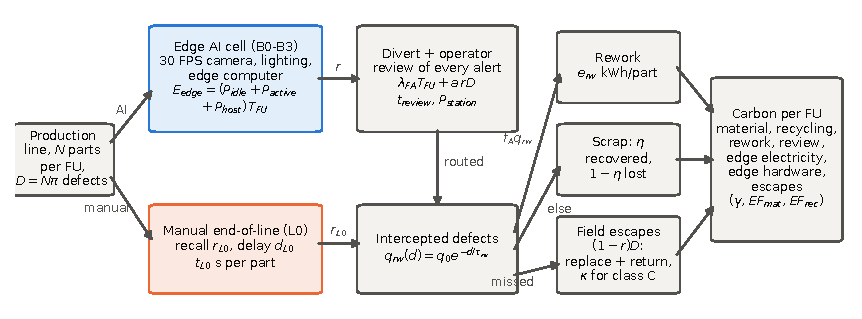
\includegraphics[width=\textwidth]{figures/fig1_system_boundary.pdf}
\caption{System boundary and flows for one functional unit. Parts are inspected either by the edge AI cell (alert policies B0--B3, detect-and-divert with operator review of every alert) or manually at the end of line (L0); without inspection (N0) all defects escape. Intercepted class-A defects are reworked with delay-dependent probability $q_{rw}(d)$, all other intercepted defects are scrapped with material recovery fraction $\eta$, and missed defects become field escapes.}
\label{fig:boundary}
\end{figure*}

\section{Accounting Model}
\subsection{Functional Unit, Regimes and Boundary}
The functional unit (FU) is $N=1{,}000$ consecutively produced parts. A line with throughput $\Theta$ [parts/h] needs $T_{FU}=N/\Theta$ hours to produce one FU. The gate-to-gate boundary (Fig.~\ref{fig:boundary}) covers inspection electricity, operator-review or manual-inspection workstations, rework electricity, the embodied carbon of unrecovered scrap, the processing burden of recovered scrap, the amortised embodied carbon of the edge hardware, and the consequences of field escapes. Facility base loads, logistics of good parts and labour-related emissions are identical across regimes, so we exclude them. The inventory also excludes the embodied carbon of the carrier board, enclosure, camera and lighting of the edge cell, of the review or inspection workstation, and of network infrastructure, as well as end-of-life treatment of the edge hardware; Section~\ref{sec:breakeven} bounds their possible effect by the multiple of the module's embodied carbon at which a conclusion would change. The study is a comparative assessment organised along the goal-and-scope elements of ISO~14040/14044~\cite{finkbeiner2006new}. Its question---what changes when a line adopts a given inspection regime---is consequential, so only flows that differ between regimes enter, and all results are differences between regimes rather than absolute footprints. Electricity carries average, location-based grid factors. Consequential studies often prefer marginal factors, which can differ substantially from average ones~\cite{hawkes2010marginal,silerevans2012marginal}; instead of committing to one, we report the grid intensity at which each conclusion reverses (Section~\ref{sec:breakeven}).

Six regimes form the main comparison. \emph{N0}: no inspection. \emph{L0}: 100\% manual end-of-line visual inspection with recall $r_{L0}$, discovery delay $d_{L0}$ and $t_{L0}$ seconds per part. \emph{B0--B3}: a continuously running edge AI cell under one of the four alert policies of~\cite{sengar2026paperA}: single-frame thresholding (B0), exponential smoothing (B1), smoothing with $k$-of-$N$ persistence (B2), and the full policy, which adds an incident latch, machine-state gating and divergence triage (B3). Section~\ref{sec:alarms} also evaluates the companion study's three textbook alarm baselines as alternatives to B3: an on-delay timer (E1), smoothing with hysteresis (E2) and decision-level fusion of visual and sensor alarms (E3). The cell diverts flagged parts automatically and an operator reviews every alert afterwards.

Several structural choices define the reference model rather than describe measured facts, and we label them as such: review queues do not delay interception (automatic diversion); recovered scrap displaces virgin material one-to-one ($s=1$, varied in Section~\ref{sec:structural}); a field escape costs the replacement part, its return freight and an optional collateral term, a lower bound that omits customer-side handling; manual recall is a literature range for visual inspection in general, not a measurement on the same parts; and detector recall is measured per image on public benchmarks.

\subsection{Defect Routing and Reworkability}
With prevalence $\pi$ the FU contains $D=N\pi$ defects in classes A (reworkable), B (scrap-prone) and C (escape-sensitive) with shares $f_A,f_B,f_C$. A regime with recall $r$ and interception delay $d$ [s] yields
\begin{align}
N_{rw} &= f_A\, r D\, q_{rw}(d), \quad q_{rw}(d) = q_0\, e^{-d/\tau_{rw}}, \label{eq:rw}\\
N_{sc} &= rD - N_{rw}, \qquad N_{esc} = (1-r)D, \label{eq:sc}
\end{align}
where $q_0$ is the zero-delay reworkability and $\tau_{rw}$ the time constant with which a defective part advances into irreversible downstream operations. By construction $N_{rw}+N_{sc}+N_{esc}=D$, and the implementation checks this identity numerically at every evaluation. For L0, $r=r_{L0}$ and $d=d_{L0}$. For an AI policy $t$, $d=d_t/f_{cam}$ with the measured mean delay $d_t$ in frames, and $r=r_{AI}(1-\delta_t)$, where $r_{AI}$ is the detector's recall and $\delta_t$ the share of the defects flagged by single-frame thresholding that policy $t$ does not flag within 15 frames of onset in the companion study's runs (an alert policy can delay or merge detections but not create them). A defect first flagged later counts as missed, a conservative choice. On MVTec~AD with independent frame scores the four policies B0--B3 flagged every sustained defect, so $\delta_t$ is centred on zero; its upper bound covers parts that stay in view for only 8 frames (Table~\ref{tab:policies}).

\subsection{Material, Workload and Energy}
Scrap mass is $M_{gr}=N_{sc}m$ for part mass $m$, of which $M_{rec}=\eta M_{gr}$ is recovered and $M_{loss}=(1-\eta)M_{gr}$ lost. We adopt the operator-load model of~\cite{sengar2026paperA}: every alert reaches the review queue. For policy $t$ the false-alert rate is $\lambda_{FA}=\lambda_t+g\,b_t$, where $\lambda_t$ [1/h] is the measured rate on good parts, $b_t$ the measured alerts per glare burst and $g$ [1/h] the rate of glare bursts. Each detected defect raises $a_t$ alerts. The operator therefore reviews $n_{ev}=\lambda_{FA}T_{FU}+a_t\,rD$ alerts per FU, giving
\begin{equation}
H = \frac{n_{ev}\, t_{review}}{3600}\ \text{[h/FU]}, \qquad \rho = \frac{n_{ev}\, t_{review}}{3600\, T_{FU}},
\end{equation}
where $t_{review}$ [s] is the time to review one alert and $\rho$ is the utilisation of a single operator; for L0, $H=N t_{L0}/3600$ and $\rho=\Theta t_{L0}/3600$; for N0, $H=0$. Electricity per FU [kWh] is
\begin{align}
E_{edge} &= (P_{idle}+P_{active}+P_{host})\,T_{FU}/1000, \\
E_{rev} &= H\,P_{station}/1000, \qquad E_{rw} = N_{rw}\,e_{rw},
\end{align}
with $E_{edge}=0$ for N0 and L0. $P_{idle}$ and $P_{active}$ are the measured idle and above-idle power of the edge computer at the camera rate (Section~\ref{sec:measure}); $P_{host}$ covers what the measurement cannot observe: the carrier board, camera and lighting of the embedded cell, and in addition the host computer when a workstation GPU is used.

\subsection{Carbon}
Carbon per FU is the sum of seven non-negative components,
\begin{equation}
\begin{split}
C ={}& [M_{loss}+(1-s)M_{rec}]\,EF_{mat} + M_{rec}EF_{rec} \\
& + \gamma\,(E_{rw}+E_{rev}+E_{edge}) + C_{hw}T_{FU}/L_{hw} \\
& + N_{esc}\,(m\,EF_{mat}+c_{ret}) + \kappa f_C N_{esc}\, m\,EF_{mat},
\end{split}
\end{equation}
where $EF_{mat}$ is the cradle-to-gate material factor, $EF_{rec}$ the processing burden of recovered scrap, $s\in[0,1]$ the share of virgin material that recovered scrap displaces ($s=1$ in the reference model: closed-loop recycling with one-to-one substitution), $\gamma$ the grid intensity, $C_{hw}$ and $L_{hw}$ the embodied carbon and service life of the edge computer (the hardware term, like $E_{edge}$, is zero for N0 and L0), and each escaped part is replaced (its material is lost) and shipped back, with return and replacement road freight $c_{ret}=2\,(m/1000)\,d_{ret}\,EF_{fr}$ at Global Logistics Emissions Council (GLEC) intensities $EF_{fr}$ [kgCO$_2$e/t-km]~\cite{glec2023}; class-C escapes add collateral damage $\kappa\, m\,EF_{mat}$. Escape consequences scale with the part; they are not a fixed penalty. For any regime $p$ and baseline $b$, savings are $\Delta X = X_b - X_p$ for $X\in\{M_{loss},E,C,H\}$. The carbon saving $\Delta C$ decomposes exactly into the seven component differences, which we verify to machine precision.

\subsection{A Decision Rule}
Every term of $C$ is either linear in the defect count $D$ (routing, material, rework, escapes, defect alerts) or independent of it (edge electricity, hardware, false-alert review, manual inspection). For any policy $p$ and baseline $b$, therefore,
\begin{equation}
\Delta C(\pi) = N\pi\,\beta - F, \qquad \pi^\star = \frac{F}{N\beta},
\label{eq:rule}
\end{equation}
where $\beta$ is the net carbon saved per defect and $F$ the fixed carbon per functional unit. For an AI policy against no inspection, $F/N = k$ is the edge cell's carbon per part,
\begin{equation}
\begin{split}
k = \frac{1}{\Theta}\Big[&\frac{\gamma(P_{idle}+P_{active}+P_{host})}{1000} + \frac{C_{hw}}{L_{hw}} \\
&+ \frac{\gamma\,\lambda_{FA}\,t_{review}P_{station}}{3.6\times10^{6}}\Big],
\end{split}
\end{equation}
and $\beta = r\,[\,m\,EF_{mat}(1+\kappa f_C)+c_{ret}-h\,]$, where $h$ is the carbon of handling an intercepted defect (scrap and recycling, rework electricity, alert review). Edge AI is carbon-beneficial exactly when $\pi\beta>k$, provided $\beta>0$. This is an analytical consequence of the model's linearity, not a new result in its own right; its value is that it turns the model into a chart. The implementation obtains $\beta$ and $F$ from two model evaluations, so~(\ref{eq:rule}) holds for every parameter set. Every term of $k$ scales as $1/\Theta$, so multiplying by $\Theta$ gives a throughput-free form: with $D_h=\pi\Theta$ defects per hour and $K=k\Theta$ the cell's carbon per hour, edge AI pays back exactly when $D_h\,\beta>K$. Because $\beta$ approaches the embodied carbon of a part as parts get heavier, the rule reads in plain terms: inspect when the defective parts the line produces per hour carry more embodied carbon than the inspection cell emits per hour.

\subsection{Parameters, Uncertainty and Verification}
Tables~\ref{tab:parameters} and~\ref{tab:policies} list all \RegistryEntries{} ledger entries with central value, bounds, unit, provenance class and source, and Table~\ref{tab:evidence} groups them by provenance class; both tables are generated from the ledger file and cannot drift from the code. The alert-policy entries are the companion study's means over its (category, replicate) units with 95\% bootstrap intervals over categories; they are imported from its pinned revision \texttt{\PaperACommit}, recomputed from its per-run result files with its own code, and checked against every value it prints. The MVTec~AD measurements with independent frame scores are the primary values; the correlated-score and held-out VisA measurements enter as alternative alert-measurement sets (Section~\ref{sec:alarms}). The review time is centred on the companion study's assumed service rate of \PaperAMu{} reviews/h and the glare rate on its assumed \PaperAGlareRate{} bursts/h. Grid intensity is centred on the 2023 value for the 27 European Union member states (EU-27) (0.242~kg/kWh~\cite{ember2024}), with the Indian fiscal-year 2022--23 weighted average (0.716~kg/kWh~\cite{cea2023}) as upper bound. Material factors come from the Inventory of Carbon and Energy (ICE)~\cite{ice2011} and the International Aluminium Institute~\cite{iai2023}, the battery-module factor from~\cite{ivl2019}, freight intensities from the GLEC Framework~\cite{glec2023} with return distances from Eurostat road-freight statistics~\cite{eurostat2026road}. The embodied carbon of the embedded module is an estimate from the Architectural Carbon Modeling Tool (ACT)~\cite{halder2025carbon,gupta2022act}; because bottom-up estimates truncate and may need about twofold upward revision~\cite{pirson2021embodied}, its upper bound is twice the estimate for the largest module considered. The workstation's embodied carbon is a manufacturer footprint~\cite{dell2021optiplex}. Defect prevalence is anchored in measured scrap rates: visual moulding defects per resin at a production injection-moulding plant (2.5--9.3\%)~\cite{nguyen2004injection} for scenario~A, and the global Li-ion manufacturing scrap rate (7.67\% in 2023, projected 4.34\% by 2030)~\cite{yu2024scrap} for scenario~C; a public semiconductor line reports 104 failures in 1{,}567 units (6.6\%)~\cite{secom2008}. Recycling burdens come from a post-industrial plastics recycling inventory~\cite{ruggeri2025postindustrial}, the electricity use of EU mechanical recycling plants~\cite{jrc2023plastics}, and industrial Li-ion recycling~\cite{machala2025recycling}. Reworkability, rework energy and manual-inspection timing remain scenario assumptions; line throughput and part mass are scenario definitions that describe the reference products, and they are varied over their ranges like the uncertain inputs. We propagate uncertainty with \MonteCarloDraws{} independent triangular draws on the ledger bounds (seed 42) and rank global sensitivity with partial rank correlation coefficients (PRCC)~\cite{marino2008methodology}, which capture monotone effects, and with first- and total-order Sobol indices, which decompose the variance of $\Delta C$ including interactions (Saltelli and Jansen estimators~\cite{saltelli2010variance,jansen1999analysis} on a scrambled Sobol sequence, 95\% bootstrap intervals). Because the ledger has no basis for joint distributions, a separate stress test imposes rank correlations on pairs of inputs (Section~\ref{sec:uncertainty}). Brent's method solves each break-even frontier ($\Delta C=0$) on a physically bounded interval; where $\Delta C$ does not change sign, we report ``none'' together with that sign. A verification script proves the structural properties of the equations above with SymPy (conservation, non-negativity of every carbon component, closure of the decomposition, monotonicity in every break-even parameter), checks their dimensions, and evaluates them against the implementation for every regime at central values and on Monte Carlo draws (relative deviation below $10^{-12}$), and checks each break-even root against its closed form. Parts of the analysis and measurement code were developed with an AI coding assistant (see the Acknowledgment); all of it is released and covered by unit, invariant and reproducibility tests.

\begin{table*}[!t]
\centering
\scriptsize
\caption{Parameter ledger (generated from \texttt{data/raw/source\_registry.csv}). Values are central [low, high]; Monte Carlo draws are triangular on these bounds. Class: M measured, P derived from our alert-policy study~\cite{sengar2026paperA}, L literature, O official dataset, D scenario definition (defines the reference product or a structural model choice), A scenario assumption; where the class differs between scenarios it is given per scenario (A, B, C). The alert-policy parameters are in Table~\ref{tab:policies}.}
\label{tab:parameters}
\setlength{\tabcolsep}{3pt}
\renewcommand{\arraystretch}{0.94}
\begin{tabular}{@{}llllllll@{}}
\toprule
Parameter & Sym. & Unit & A: Precision & B: Machined metal & C: High-value & Cl. & Source \\
\midrule
\multicolumn{8}{@{}l}{\emph{Global and edge-cell parameters}} \\
functional unit & $N$ & parts & \multicolumn{3}{c}{1{,}000} & D & -- \\
camera fps & $f_{cam}$ & frames/s & \multicolumn{3}{c}{30} & D & -- \\
edge idle power & $P_{idle}$ & W & \multicolumn{3}{c}{3.11 [3.11, 3.16]} & M & this study \\
edge active power & $P_{active}$ & W & \multicolumn{3}{c}{0.846 [0.819, 1.04]} & M & this study \\
host power & $P_{host}$ & W & \multicolumn{3}{c}{12 [5, 30]} & A & -- \\
edge embodied carbon & $C_{hw}$ & kgCO$_2$e & \multicolumn{3}{c}{168 [54.6, 461]} & L & \cite{halder2025carbon,gupta2022act,pirson2021embodied} \\
edge lifetime hours & $L_{hw}$ & h & \multicolumn{3}{c}{20{,}000 [10{,}000, 43{,}800]} & L & \cite{halder2025carbon} \\
review station power & $P_{station}$ & W & \multicolumn{3}{c}{85 [65, 120]} & A & -- \\
grid carbon factor & $\gamma$ & kgCO$_2$e/kWh & \multicolumn{3}{c}{0.242 [0.1, 0.716]} & O & \cite{ember2024,cea2023} \\
manual inspection recall & $r_{L0}$ & fraction & \multicolumn{3}{c}{0.750 [0.700, 0.800]} & L & \cite{see2012visual} \\
collateral multiplier & $\kappa$ & -- & \multicolumn{3}{c}{1 [0, 5]} & A & -- \\
review time & $t_{review}$ & s & \multicolumn{3}{c}{60 [30, 90]} & P & \cite{sengar2026paperA} \\
glare burst rate & $g$ & bursts/h & \multicolumn{3}{c}{30 [10, 60]} & A & \cite{sengar2026paperA} \\
ai recall & $r_{AI}$ & fraction & \multicolumn{3}{c}{0.792 [0.137, 1.00]} & M & this study \\
cry wolf strength & $\omega$ & -- & \multicolumn{3}{c}{0} & L & \cite{bliss1995probability,wickens2009false} \\
recycled substitution ratio & $s$ & fraction & \multicolumn{3}{c}{1.00} & D & -- \\
freight carbon intensity & $EF_{fr}$ & kgCO$_2$e/t-km & \multicolumn{3}{c}{0.195 [0.115, 0.8]} & L & \cite{glec2023} \\
return distance & $d_{ret}$ & km & \multicolumn{3}{c}{142 [97.5, 594]} & O & \cite{eurostat2026road} \\
\midrule
\multicolumn{8}{@{}l}{\emph{Scenario parameters}} \\
line throughput & $\Theta$ & parts/h & 1{,}800 [1{,}200, 3{,}600] & 120 [60, 240] & 30 [15, 60] & D & -- \\
defect prevalence & $\pi$ & fraction & 0.0460 [0.0250, 0.0930] & 0.0300 [0.0150, 0.0500] & 0.0767 [0.0434, 0.100] & L/A/L & \cite{nguyen2004injection,yu2024scrap} \\
part mass & $m$ & kg & 0.015 [0.01, 0.02] & 1.25 [1, 1.6] & 14.5 [12, 18] & D & -- \\
material carbon factor & $EF_{mat}$ & kgCO$_2$e/kg & 3.76 [3.31, 7.62] & 9.16 [1.81, 14.8] & 13.5 [8.91, 27.2] & L & \cite{ice2011,iai2023,ivl2019} \\
material recovery fraction & $\eta$ & fraction & 0.400 [0.300, 0.500] & 0.810 [0.760, 0.860] & 0.600 [0.450, 0.750] & A/L/A & \cite{allwood2011material,iai2024recycling} \\
recycling burden & $EF_{rec}$ & kgCO$_2$e/kg & 0.152 [0.073, 0.5] & 1.81 [1.45, 2.12] & 2.8 [1, 6.1] & L & \cite{ruggeri2025postindustrial,jrc2023plastics,ice2011,machala2025recycling} \\
rework energy & $e_{rw}$ & kWh/part & 0.05 [0.03, 0.08] & 1.8 [1.2, 2.5] & 5.5 [3.8, 7.5] & A & -- \\
base reworkability & $q_0$ & fraction & 0.900 [0.800, 0.950] & 0.850 [0.750, 0.920] & 0.700 [0.600, 0.800] & A & -- \\
reworkability time constant & $\tau_{rw}$ & s & 30 [15, 60] & 60 [30, 120] & 20 [10, 40] & A & -- \\
manual discovery delay & $d_{L0}$ & s & 60 [30, 120] & 120 [60, 300] & 600 [300, 1{,}200] & A & -- \\
manual inspection time & $t_{L0}$ & s/part & 2 [1, 4] & 10 [5, 20] & 30 [15, 60] & A & -- \\
defect class shares & $f_A{:}f_B{:}f_C$ & -- & 0.70:0.25:0.05 & 0.60:0.35:0.05 & 0.40:0.40:0.20 & A & -- \\
\bottomrule
\end{tabular}
\end{table*}


\begin{table}[!t]
\centering
\scriptsize
\caption{Evidence behind the ledger: entries per provenance class (primary analysis; the correlated-score variant adds the entries in brackets) and the parameters they cover. A parameter appears under several classes when its class differs between scenarios.}
\label{tab:evidence}
\setlength{\tabcolsep}{3pt}
\begin{tabular}{@{}lr>{\raggedright\arraybackslash}p{0.52\columnwidth}@{}}
\toprule
Class & Entries & Parameters \\
\midrule
Measured (M) & 5 & ai recall, edge active power, edge idle power \\
Imported from~\cite{sengar2026paperA} (P) & 36 [+105] & alerts per defect, detection delay, glare alerts per burst, nominal false alarm rate, recall loss, review time \\
Literature (L) & 16 & cry wolf strength, defect prevalence, edge embodied carbon, edge lifetime hours, freight carbon intensity, manual inspection recall, material carbon factor, material recovery fraction, recycling burden \\
Official data (O) & 2 & grid carbon factor, return distance \\
Scenario definition (D) & 9 & camera fps, functional unit, line throughput, part mass, recycled substitution ratio \\
Scenario assumption (A) & 23 & base reworkability, collateral multiplier, defect prevalence, glare burst rate, host power, manual discovery delay, manual inspection time, material recovery fraction, review station power, rework energy, reworkability time constant \\
\bottomrule
\end{tabular}
\end{table}


\begin{table*}[!t]
\centering
\scriptsize
\caption{Alert policies of the companion study~\cite{sengar2026paperA} (revision \texttt{4752116}), measured on PatchCore scores of 7 MVTec~AD categories and, with the policy frozen, 12 held-out VisA categories: mean over 21 (MVTec~AD) or 36 (VisA) (category, replicate) units [95\% bootstrap interval over categories], recomputed from its per-run results and checked against its printed values. B0 thresholds every frame, B1 adds exponential smoothing, B2 adds $k$-of-$N$ persistence and B3 is the full policy (incident latch, machine-state gating, divergence triage); E1--E3 are textbook alarm baselines (on-delay timer, EMA with hysteresis, decision-level fusion). $\delta_t$ is the share of the sustained defects flagged by single-frame thresholding that policy $t$ does not flag within 15 frames of onset; for MVTec~AD with independent scores its upper bound also covers parts visible for only 8 frames. Correlated: AR(1) frame scores with $\rho=0.9$.}
\label{tab:policies}
\setlength{\tabcolsep}{3pt}
\renewcommand{\arraystretch}{0.82}
\begin{tabular}{@{}lccccccc@{}}
\toprule
Quantity & B0 & B1 & B2 & B3 & E1 & E2 & E3 \\
\midrule
\multicolumn{8}{@{}l}{\emph{MVTec~AD, independent frame scores (primary)}} \\
False alerts on good parts $\lambda_t$ (1/h) & \shortstack{4{,}616\\[-1pt]{\tiny[1{,}557, 8{,}374]}} & \shortstack{40.6\\[-1pt]{\tiny[0, 114]}} & 0 & 0 & \shortstack{5.14\\[-1pt]{\tiny[0, 15.4]}} & \shortstack{3.43\\[-1pt]{\tiny[0, 6.86]}} & \shortstack{5.14\\[-1pt]{\tiny[0, 15.4]}} \\
Alerts per 1--3 frame glare burst $b_t$ & \shortstack{2.63\\[-1pt]{\tiny[2.24, 3.14]}} & \shortstack{4.27\\[-1pt]{\tiny[3.12, 5.24]}} & \shortstack{5.66\\[-1pt]{\tiny[3.64, 7.33]}} & \shortstack{0.664\\[-1pt]{\tiny[0.438, 0.832]}} & \shortstack{0.0286\\[-1pt]{\tiny[0.00833, 0.0488]}} & \shortstack{0.590\\[-1pt]{\tiny[0.354, 0.863]}} & \shortstack{0.0286\\[-1pt]{\tiny[0.00833, 0.0488]}} \\
Alerts per defect episode $a_t$ & \shortstack{138\\[-1pt]{\tiny[125, 150]}} & \shortstack{149\\[-1pt]{\tiny[143, 155]}} & \shortstack{154\\[-1pt]{\tiny[149, 158]}} & 1.00 & \shortstack{1.23\\[-1pt]{\tiny[1.02, 1.47]}} & \shortstack{1.58\\[-1pt]{\tiny[0.589, 2.93]}} & \shortstack{0.982\\[-1pt]{\tiny[0.946, 1.00]}} \\
Mean detection delay $d_t$ (frames) & \shortstack{0.101\\[-1pt]{\tiny[0.0179, 0.220]}} & \shortstack{0.583\\[-1pt]{\tiny[0.208, 0.988]}} & \shortstack{3.65\\[-1pt]{\tiny[3.22, 4.18]}} & \shortstack{3.65\\[-1pt]{\tiny[3.22, 4.18]}} & \shortstack{3.94\\[-1pt]{\tiny[2.92, 5.17]}} & \shortstack{0.393\\[-1pt]{\tiny[0.0774, 0.804]}} & \shortstack{3.94\\[-1pt]{\tiny[2.92, 5.17]}} \\
Recall loss $\delta_t$ & 0 & \shortstack{0\\[-1pt]{\tiny[0, 0.00238]}} & \shortstack{0\\[-1pt]{\tiny[0, 0.0262]}} & \shortstack{0\\[-1pt]{\tiny[0, 0.0262]}} & \shortstack{0.0417\\[-1pt]{\tiny[0, 0.125]}} & \shortstack{0\\[-1pt]{\tiny[0, 0.00238]}} & \shortstack{0.0417\\[-1pt]{\tiny[0, 0.125]}} \\
\multicolumn{8}{@{}l}{\emph{MVTec~AD, correlated frame scores ($\rho=0.9$)}} \\
False alerts on good parts $\lambda_t$ (1/h) & \shortstack{4{,}615\\[-1pt]{\tiny[1{,}556, 8{,}298]}} & \shortstack{2{,}097\\[-1pt]{\tiny[435, 3{,}808]}} & \shortstack{2{,}438\\[-1pt]{\tiny[468, 4{,}504]}} & \shortstack{189\\[-1pt]{\tiny[41.7, 342]}} & \shortstack{300\\[-1pt]{\tiny[103, 526]}} & \shortstack{105\\[-1pt]{\tiny[12.0, 214]}} & \shortstack{300\\[-1pt]{\tiny[103, 526]}} \\
Alerts per 1--3 frame glare burst $b_t$ & \shortstack{2.60\\[-1pt]{\tiny[2.21, 3.09]}} & \shortstack{4.62\\[-1pt]{\tiny[3.50, 5.61]}} & \shortstack{6.05\\[-1pt]{\tiny[4.23, 7.62]}} & \shortstack{0.625\\[-1pt]{\tiny[0.458, 0.748]}} & \shortstack{0.0619\\[-1pt]{\tiny[0.0250, 0.102]}} & \shortstack{0.663\\[-1pt]{\tiny[0.446, 0.925]}} & \shortstack{0.0619\\[-1pt]{\tiny[0.0250, 0.102]}} \\
Alerts per defect episode $a_t$ & \shortstack{136\\[-1pt]{\tiny[121, 149]}} & \shortstack{141\\[-1pt]{\tiny[126, 152]}} & \shortstack{146\\[-1pt]{\tiny[134, 156]}} & \shortstack{1.07\\[-1pt]{\tiny[0.940, 1.23]}} & \shortstack{1.58\\[-1pt]{\tiny[1.32, 1.91]}} & \shortstack{1.79\\[-1pt]{\tiny[1.18, 2.47]}} & \shortstack{1.04\\[-1pt]{\tiny[0.917, 1.22]}} \\
Mean detection delay $d_t$ (frames) & \shortstack{0.185\\[-1pt]{\tiny[0, 0.381]}} & \shortstack{0.766\\[-1pt]{\tiny[0.137, 1.52]}} & \shortstack{3.75\\[-1pt]{\tiny[3.08, 4.56]}} & \shortstack{3.75\\[-1pt]{\tiny[3.08, 4.56]}} & \shortstack{3.38\\[-1pt]{\tiny[2.74, 4.29]}} & \shortstack{0.678\\[-1pt]{\tiny[0.101, 1.42]}} & \shortstack{3.38\\[-1pt]{\tiny[2.74, 4.29]}} \\
Recall loss $\delta_t$ & 0 & \shortstack{0.0128\\[-1pt]{\tiny[0, 0.0272]}} & \shortstack{0.0255\\[-1pt]{\tiny[0.00595, 0.0527]}} & \shortstack{0.0255\\[-1pt]{\tiny[0.00595, 0.0527]}} & \shortstack{0.0255\\[-1pt]{\tiny[0.00595, 0.0527]}} & \shortstack{0\\[-1pt]{\tiny[0, 0.0204]}} & \shortstack{0.0255\\[-1pt]{\tiny[0.00595, 0.0527]}} \\
\multicolumn{8}{@{}l}{\emph{VisA (held out), independent frame scores}} \\
False alerts on good parts $\lambda_t$ (1/h) & \shortstack{2{,}029\\[-1pt]{\tiny[1{,}078, 3{,}093]}} & \shortstack{192\\[-1pt]{\tiny[0, 551]}} & \shortstack{10.3\\[-1pt]{\tiny[0, 28.3]}} & \shortstack{1.67\\[-1pt]{\tiny[0, 4.67]}} & 0 & \shortstack{3.33\\[-1pt]{\tiny[0, 8.67]}} & 0 \\
Alerts per 1--3 frame glare burst $b_t$ & \shortstack{2.28\\[-1pt]{\tiny[2.12, 2.46]}} & \shortstack{3.63\\[-1pt]{\tiny[2.90, 4.28]}} & \shortstack{4.45\\[-1pt]{\tiny[3.15, 5.57]}} & \shortstack{0.547\\[-1pt]{\tiny[0.392, 0.680]}} & \shortstack{0.00764\\[-1pt]{\tiny[0.00347, 0.0125]}} & \shortstack{0.735\\[-1pt]{\tiny[0.468, 0.985]}} & \shortstack{0.00764\\[-1pt]{\tiny[0.00347, 0.0125]}} \\
Alerts per defect episode $a_t$ & \shortstack{82.1\\[-1pt]{\tiny[59.1, 105]}} & \shortstack{101\\[-1pt]{\tiny[69.2, 129]}} & \shortstack{112\\[-1pt]{\tiny[79.3, 141]}} & \shortstack{1.34\\[-1pt]{\tiny[0.910, 1.80]}} & \shortstack{0.924\\[-1pt]{\tiny[0.628, 1.21]}} & \shortstack{1.74\\[-1pt]{\tiny[0.635, 3.12]}} & \shortstack{0.785\\[-1pt]{\tiny[0.587, 0.951]}} \\
Mean detection delay $d_t$ (frames) & \shortstack{1.30\\[-1pt]{\tiny[0.549, 2.28]}} & \shortstack{2.73\\[-1pt]{\tiny[1.59, 4.09]}} & \shortstack{5.75\\[-1pt]{\tiny[4.58, 7.08]}} & \shortstack{5.75\\[-1pt]{\tiny[4.58, 7.08]}} & \shortstack{6.13\\[-1pt]{\tiny[5.08, 7.34]}} & \shortstack{1.98\\[-1pt]{\tiny[0.920, 3.30]}} & \shortstack{6.13\\[-1pt]{\tiny[5.08, 7.34]}} \\
Recall loss $\delta_t$ & 0 & \shortstack{0.0933\\[-1pt]{\tiny[0, 0.249]}} & \shortstack{0.229\\[-1pt]{\tiny[0.0556, 0.431]}} & \shortstack{0.229\\[-1pt]{\tiny[0.0556, 0.431]}} & \shortstack{0.476\\[-1pt]{\tiny[0.253, 0.715]}} & \shortstack{0.0863\\[-1pt]{\tiny[0, 0.242]}} & \shortstack{0.476\\[-1pt]{\tiny[0.253, 0.715]}} \\
\multicolumn{8}{@{}l}{\emph{VisA (held out), correlated frame scores ($\rho=0.9$)}} \\
False alerts on good parts $\lambda_t$ (1/h) & \shortstack{1{,}854\\[-1pt]{\tiny[974, 2{,}788]}} & \shortstack{1{,}155\\[-1pt]{\tiny[457, 2{,}047]}} & \shortstack{1{,}336\\[-1pt]{\tiny[507, 2{,}397]}} & \shortstack{111\\[-1pt]{\tiny[46.3, 189]}} & \shortstack{126\\[-1pt]{\tiny[65.0, 192]}} & \shortstack{122\\[-1pt]{\tiny[63.3, 181]}} & \shortstack{126\\[-1pt]{\tiny[65.0, 192]}} \\
Alerts per 1--3 frame glare burst $b_t$ & \shortstack{2.30\\[-1pt]{\tiny[2.11, 2.52]}} & \shortstack{3.85\\[-1pt]{\tiny[3.15, 4.49]}} & \shortstack{4.86\\[-1pt]{\tiny[3.74, 5.88]}} & \shortstack{0.545\\[-1pt]{\tiny[0.426, 0.647]}} & \shortstack{0.0319\\[-1pt]{\tiny[0.0173, 0.0472]}} & \shortstack{0.794\\[-1pt]{\tiny[0.562, 1.02]}} & \shortstack{0.0319\\[-1pt]{\tiny[0.0173, 0.0472]}} \\
Alerts per defect episode $a_t$ & \shortstack{82.9\\[-1pt]{\tiny[60.4, 105]}} & \shortstack{87.7\\[-1pt]{\tiny[63.8, 111]}} & \shortstack{97.2\\[-1pt]{\tiny[72.4, 120]}} & \shortstack{1.60\\[-1pt]{\tiny[1.34, 1.83]}} & \shortstack{2.18\\[-1pt]{\tiny[1.80, 2.51]}} & \shortstack{2.09\\[-1pt]{\tiny[1.42, 2.69]}} & \shortstack{1.50\\[-1pt]{\tiny[1.26, 1.71]}} \\
Mean detection delay $d_t$ (frames) & \shortstack{2.49\\[-1pt]{\tiny[1.23, 3.86]}} & \shortstack{3.57\\[-1pt]{\tiny[2.31, 4.92]}} & \shortstack{5.31\\[-1pt]{\tiny[4.59, 6.06]}} & \shortstack{5.31\\[-1pt]{\tiny[4.59, 6.06]}} & \shortstack{4.75\\[-1pt]{\tiny[4.01, 5.59]}} & \shortstack{2.59\\[-1pt]{\tiny[1.39, 3.86]}} & \shortstack{4.75\\[-1pt]{\tiny[4.01, 5.59]}} \\
Recall loss $\delta_t$ & 0 & \shortstack{0.157\\[-1pt]{\tiny[0.0591, 0.283]}} & \shortstack{0.294\\[-1pt]{\tiny[0.157, 0.451]}} & \shortstack{0.294\\[-1pt]{\tiny[0.157, 0.451]}} & \shortstack{0.293\\[-1pt]{\tiny[0.157, 0.451]}} & \shortstack{0.0960\\[-1pt]{\tiny[0, 0.215]}} & \shortstack{0.293\\[-1pt]{\tiny[0.157, 0.451]}} \\
\bottomrule
\end{tabular}
\end{table*}


\section{Edge Inference Power Measurement}
\label{sec:measure}
\subsection{Workload, Platforms and Protocol}
The workload is the PatchCore detector of~\cite{sengar2026paperA}: an ImageNet-pretrained ResNet-18, layer-2 and layer-3 features pooled to $28\times28\times384$ patch descriptors, exact 1-nearest-neighbour search against a memory bank, and the Gaussian-smoothed maximum as image score, for $224\times224$ colour (RGB) frames at batch size~1. The bank holds $\PaperABank$ real patch features, the bank size of the companion study's latency benchmark, selected by greedy coreset from \BenchFitImages{} good \BenchCategory{} training images, and the stream cycles through \BenchFrames{} real \BenchCategory{} test frames, good and defective. We measured four cumulative stages: the model alone; plus score thresholding; plus a temporal policy (exponential smoothing, $k$-of-$N$ persistence and cooldown; a simplified 3-of-5 version of the companion policy, whose per-frame cost is below the measurement resolution either way); and the full pipeline with SQLite write-ahead-log event persistence and JavaScript Object Notation (JSON) serialisation. Each stage ran paced at the line rate of \BenchFps{} frames per second (FPS) for \BenchWindow~s windows, in \BenchRepeats{} repeats with a seeded random stage order, and a 15~s idle window preceded every repeat. Power was sampled at 20~Hz and integrated over each window; we report the median across repeats, with the minimum and maximum as bounds.

We ran the protocol on two platforms. The primary one is an embedded \JetsonModel{} module (\JetsonLft, TensorRT \JetsonTensorRT, \JetsonPowerMode{} power mode), the class of device typically mounted beside a line. The whole scoring path---backbone, nearest-neighbour search against the bank, bilinear upsampling, Gaussian filter and maximum---is exported as one Open Neural Network Exchange (ONNX) graph, checked against the PyTorch reference scorer before export, and compiled to a TensorRT engine; every frame is copied to the device and its score copied back. The module's INA3221 monitor reports its total input power (VDD\_IN), which covers the central processing unit (CPU), GPU, memory and system-on-chip (SoC), so on this platform only the carrier board, camera and lighting enter through $P_{host}$. Half precision (16-bit floating point, FP16) is the deployed precision: its scores deviate from the single-precision (FP32) reference by at most \JetsonPcHalfMaxRelErr\% and every alert decision on the \BenchFrames{} frames is identical. For comparison we also measured FP32 and a second detector, PaDiM~\cite{defard2021padim} (Section~\ref{sec:detector}). The second platform is a workstation GPU (NVIDIA \GpuName{}, PyTorch \TorchVersion{} in FP32, CUDA \CudaRuntime, Windows Subsystem for Linux, WSL2), measured with the NVIDIA Management Library (NVML), which observes the GPU only. Every stage window there contains at least \StageReadingsMin{} distinct sensor readings (idle windows at least \IdleReadingsMin). We logged the NVML cumulative energy counter but do not use it: under WSL2 it reported \CounterIdleMinW--\CounterIdleMaxW~W at idle, inconsistent with the power sensor. The workstation GPU also drives the host desktop; windows disturbed by desktop activity remain in the bounds and in the raw data.

\subsection{Results}
Fig.~\ref{fig:energy} shows that the pipeline stages are indistinguishable on the workstation: median total power ranges over \StageSpreadW~W at \BenchFps~FPS. Thresholding, the temporal policy and event logging add no measurable energy, consistent with the sub-millisecond policy step reported in~\cite{sengar2026paperA}. The whole Jetson module draws a median of \JetsonFullTotalPower~W while running the full FP16 pipeline; referenced to the idle window of the same repeat, the median above-idle power is \JetsonFullActivePower~W (median idle \JetsonIdlePower~W; medians of different windows need not add up), or \JetsonPcHalfFrameMJ~mJ per frame above idle. FP32 costs \JetsonPcFullFrameMJ~mJ and PaDiM \JetsonPdHalfFrameMJ~mJ (FP16) per frame. The workstation GPU alone draws \FullTotalPower~W (\FullActivePower~W above idle, bounds \FullActivePowerMin--\FullActivePowerMax~W), or \WorkstationFrameMJ~mJ per frame, \FrameEnergyRatio{} times the Jetson's. Unpaced, the Jetson reaches \JetsonPcHalfMaxFps~FPS in FP16 and the workstation \FullMaxFps~FPS, so both sustain the line rate with margin; the paced per-frame latency on the workstation has a median of \FullLatencyMs~ms, comparable to the \PaperAVisionLatency~ms paced vision stage reported in~\cite{sengar2026paperA}. With the assumed $P_{host}$ allowance (\HostPowerCentral~W) the embedded cell draws about \JetsonCellPower~W, of which the module is \JetsonComputeShare\%: under this assumption camera and lighting, not inference, dominate the cell's electricity. The workstation cell draws about \WsCellPower~W. On the embedded platform $E_{edge}$ is between \PrecEdgeKWh{} and \HiValEdgeKWh~kWh per FU, depending on how long the line takes to produce one FU, and the edge cell's carbon (electricity and hardware) is \PlatformCarbonRatio{} times lower than with the workstation in every scenario. No conclusion of Section~\ref{sec:results} depends on the platform: $\Delta C$ against manual inspection changes by at most \PlatformDeltaCMax\%.

\begin{figure*}[!t]
\centering
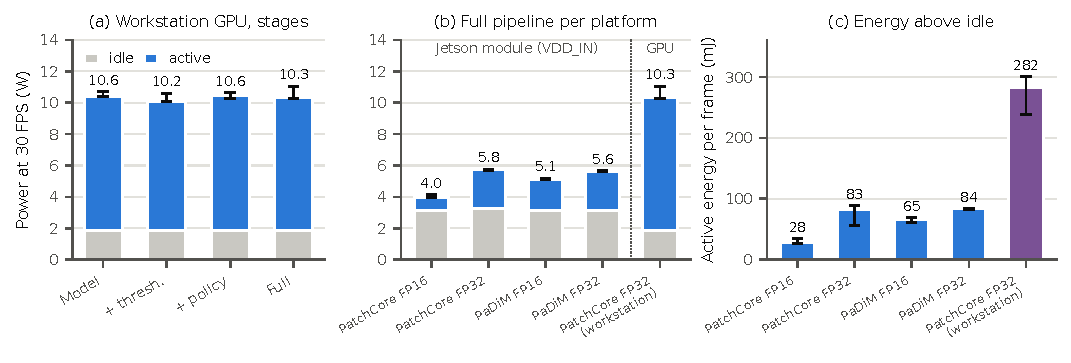
\includegraphics[width=\textwidth]{figures/fig2_measured_edge_energy.pdf}
\caption{Measured edge power at \BenchFps~FPS (median over \BenchRepeats{} repeats of \BenchWindow~s windows; whiskers min--max). (a) Cumulative pipeline stages on the workstation GPU (NVML). (b) Full pipeline for each measured configuration: whole \JetsonModel{} module (INA3221 VDD\_IN) and workstation GPU only. (c) Active energy per frame above idle.}
\label{fig:energy}
\end{figure*}

\section{Detector Operating Points}
\label{sec:detector}
The same detector, fitted per category, provides the recall the accounting needs. To avoid resting it on one benchmark, we evaluate all \DetMvtecCategories{} MVTec~AD categories~\cite{bergmann2021mvtec} and all \DetVisaCategories{} VisA categories~\cite{zou2022visa} (official one-class split), whose multi-instance and printed-circuit-board (PCB) images are closer to production imagery, with PatchCore and, as a second detector, PaDiM~\cite{defard2021padim} (ResNet-18 layers 1--3, 100 randomly retained channels, one Gaussian per patch position). For each category and \DetSeeds{} random splits, 60\% of the good training images fit the detector (PatchCore bank: 10\% coreset, \DetBankMin--\DetBankMax{} patches), 20\% calibrate thresholds, and the remaining 20\% join the good test images as nominal evaluation data (at least \DetGoodEvalMin{} images per category); defective test images give per-part recall. Table~\ref{tab:detector} and Fig.~\ref{fig:detector} (left) report the results. PatchCore reaches a median area under the receiver operating characteristic curve (AUROC) of \DetPcMvtecAurocMedian{} on MVTec~AD and \DetPcVisaAurocMedian{} on VisA, and is more accurate than PaDiM in \DetPcBeatsPdAuroc{} of \DetCategories{} categories (PaDiM: \DetPdMvtecAurocMedian{} and \DetPdVisaAurocMedian). At the 99th percentile of the calibration scores (q99), PatchCore's median recall is \DetPcMvtecRecallMedian{} on MVTec~AD but \DetPcVisaRecallMedian{} on VisA (PaDiM: \DetPdMvtecRecallMedian{} and \DetPdVisaRecallMedian), and over all categories it ranges from \DetRecallMin{} (\DetWorstCategory) to \DetRecallMax{} at false-positive rates of \DetFprMin--\DetFprMax\%; the false-positive rate at q99 exceeds the nominal 1\% in most categories because good test images score higher than good training images. The ledger's detector recall $r_{AI}$ is PatchCore's median over all \DetCategories{} categories, \DetRecallMedian, with the category range as bounds; it is deliberately the recall of a strict, alarm-budget style threshold, and Section~\ref{sec:thresholds} shows how much a carbon-aware threshold recovers. Recall is measured per image; a station that sees a part in several frames may catch more defects but also raises more false alerts, and nominal-image counts limit the resolution of false-positive rates to about one percent. PaDiM also costs more energy per frame on the Jetson (\JetsonPdHalfFrameMJ{} vs \JetsonPcHalfFrameMJ~mJ in FP16): on both counts the detector choice matters more than its power draw.

\begin{table}[!t]
\centering
\scriptsize
\caption{Measured detector operating points (mean over three splits): AUROC and per-part recall at the 99th percentile of the calibration scores (q99) for PatchCore (PC) and PaDiM (PD), and the in-sample carbon-optimal FPR and recall of a one-shot PatchCore station for scenario~C.}
\label{tab:detector}
\setlength{\tabcolsep}{2.6pt}
\begin{tabular}{@{}lcccccc@{}}
\toprule
 & \multicolumn{2}{c}{AUROC} & \multicolumn{2}{c}{Recall (q99)} & \multicolumn{2}{c}{Optimum (C)} \\
\cmidrule(lr){2-3}\cmidrule(lr){4-5}\cmidrule(l){6-7}
Category & PC & PD & PC & PD & FPR$^\star$ & Recall$^\star$ \\
\midrule
\multicolumn{7}{@{}l}{\emph{MVTec AD}} \\
bottle & 1.000 & 0.998 & 1.00 & 0.98 & 0.011 & 1.00 \\
cable & 0.988 & 0.861 & 0.82 & 0.35 & 0.269 & 1.00 \\
capsule & 0.968 & 0.885 & 0.79 & 0.46 & 0.393 & 1.00 \\
carpet & 0.985 & 0.985 & 0.96 & 0.94 & 0.548 & 0.99 \\
grid & 0.936 & 0.902 & 0.67 & 0.66 & 0.568 & 0.97 \\
hazelnut & 1.000 & 0.922 & 0.99 & 0.63 & 0.042 & 1.00 \\
leather & 1.000 & 1.000 & 1.00 & 1.00 & 0.091 & 1.00 \\
metal nut & 0.992 & 0.982 & 0.96 & 0.94 & 0.091 & 0.99 \\
pill & 0.917 & 0.804 & 0.52 & 0.26 & 0.554 & 0.96 \\
screw & 0.961 & 0.752 & 0.60 & 0.13 & 0.527 & 1.00 \\
tile & 0.997 & 0.950 & 0.96 & 0.42 & 0.207 & 1.00 \\
toothbrush & 0.959 & 0.937 & 0.94 & 0.84 & 0.417 & 1.00 \\
transistor & 0.994 & 0.890 & 0.93 & 0.32 & 0.114 & 1.00 \\
wood & 0.996 & 0.988 & 0.91 & 0.91 & 0.150 & 1.00 \\
zipper & 0.980 & 0.910 & 0.97 & 0.49 & 0.471 & 0.99 \\
\multicolumn{7}{@{}l}{\emph{VisA}} \\
candle & 0.965 & 0.875 & 0.56 & 0.14 & 0.349 & 0.99 \\
capsules & 0.718 & 0.638 & 0.38 & 0.09 & 0.546 & 0.76 \\
cashew & 0.935 & 0.874 & 0.57 & 0.13 & 0.510 & 0.98 \\
chewinggum & 0.986 & 0.978 & 0.94 & 0.85 & 0.474 & 0.99 \\
fryum & 0.903 & 0.903 & 0.61 & 0.18 & 0.419 & 0.93 \\
macaroni1 & 0.904 & 0.820 & 0.31 & 0.10 & 0.477 & 0.97 \\
macaroni2 & 0.717 & 0.708 & 0.14 & 0.01 & 0.529 & 0.82 \\
pcb1 & 0.943 & 0.922 & 0.57 & 0.34 & 0.450 & 0.99 \\
pcb2 & 0.948 & 0.830 & 0.57 & 0.17 & 0.493 & 1.00 \\
pcb3 & 0.922 & 0.724 & 0.47 & 0.14 & 0.519 & 0.98 \\
pcb4 & 0.994 & 0.955 & 0.92 & 0.46 & 0.129 & 1.00 \\
pipe fryum & 0.989 & 0.918 & 0.77 & 0.46 & 0.340 & 1.00 \\
\bottomrule
\end{tabular}
\end{table}


\section{Results}
\label{sec:results}
\subsection{Regime Comparison}
Table~\ref{tab:regimes} and Fig.~\ref{fig:regimes} summarise the six regimes at central parameter values. Relative to manual inspection, the full policy B3 reduces carbon by \PrecRelCarbonReduction\%, \MetalRelCarbonReduction\% and \HiValRelCarbonReduction\% in scenarios A, B and C ($\Delta C=\PrecDeltaCvsLZero$, \MetalDeltaCvsLZero{} and \HiValDeltaCvsLZero~\kgce{} per FU) and reduces unrecovered material ($\Delta M=\PrecDeltaMvsLZero$, \MetalDeltaMvsLZero{} and \HiValDeltaMvsLZero~kg). It uses \emph{more} electricity ($\Delta E=\PrecDeltaEvsLZero$, $\MetalDeltaEvsLZero$ and $\HiValDeltaEvsLZero$~kWh), almost all of it rework electricity: prompt interception keeps defects reworkable that manual end-of-line inspection finds too late. It also needs more operator time than manual inspection ($\Delta H=\PrecDeltaHvsLZero$, $\MetalDeltaHvsLZero$ and $\HiValDeltaHvsLZero$~h), because every alert, including those caused by glare, takes a full review. Without the incident latch the picture changes completely: single-frame thresholding (B0) produces $\rho=\PrecRhoBZero$, \MetalRhoBZero{} and \HiValRhoBZero{}, i.e.\ it would need \PrecReviewersBZero, \MetalReviewersBZero{} and \HiValReviewersBZero{} reviewers. In scenario~A the resulting review-station electricity makes B0 emit more than manual inspection (\PrecCarbonBZero{} vs \PrecCarbonLZero~\kgce{}). With independent frame scores B3 stays below one reviewer in scenarios B and C but needs \PrecReviewersBThree{} in scenario~A ($\rho=\PrecRhoBThree$), whose defect rate exceeds the roughly \PaperALoadCross{} defect episodes per hour that the scenario analysis of~\cite{sengar2026paperA} gives as the limit for one reviewer.

\begin{table*}[!t]
\centering
\scriptsize
\caption{Outcomes per functional unit (1{,}000 parts) at central parameter values. $\rho$ is single-operator utilization (values $\geq 1$ require additional operators). Carbon includes material, recycling, rework, review, edge electricity, amortized edge hardware and field-escape terms.}
\label{tab:regimes}
\setlength{\tabcolsep}{4pt}
\begin{tabular}{@{}llrrrrrrrrr@{}}
\toprule
Scenario & Regime & $r$ & $d$ (s) & $N_{rw}$ & $N_{esc}$ & $M_{loss}$ (kg) & $E$ (kWh) & $E_{edge}$ (kWh) & $H$ (h) / $\rho$ & $C$ (kgCO$_2$e) \\
\midrule
A: Precision & N0 no inspection & 0.00 & 0 & 0.00 & 46.00 & 0 & 0 & 0 & 0 / 0.00 & 2.76 \\
 & L0 manual EoL & 0.75 & 60 & 2.94 & 11.50 & 0.284 & 0.194 & 0 & 0.556 / 1.00 & 1.83 \\
 & B0 single-frame threshold & 0.79 & 0.00337 & 22.95 & 9.57 & 0.121 & 12.0 & 0.00886 & 127 / 228.69 & 3.94 \\
 & B1 smoothing & 0.79 & 0.0194 & 22.94 & 9.57 & 0.121 & 8.99 & 0.00886 & 92.2 / 165.90 & 3.22 \\
 & B2 smoothing + k-of-N & 0.79 & 0.122 & 22.86 & 9.57 & 0.122 & 9.23 & 0.00886 & 95.1 / 171.09 & 3.28 \\
 & B3 full policy (latch) & 0.79 & 0.122 & 22.86 & 9.57 & 0.122 & 1.22 & 0.00886 & 0.792 / 1.43 & 1.35 \\
\midrule
B: Machined metal & N0 no inspection & 0.00 & 0 & 0.00 & 30.00 & 0 & 0 & 0 & 0 / 0.00 & 363 \\
 & L0 manual EoL & 0.75 & 120 & 1.55 & 7.50 & 4.97 & 3.03 & 0 & 2.78 / 0.33 & 175 \\
 & B0 single-frame threshold & 0.79 & 0.00337 & 12.12 & 6.24 & 2.77 & 82.0 & 0.133 & 707 / 84.79 & 142 \\
 & B1 smoothing & 0.79 & 0.0194 & 12.11 & 6.24 & 2.77 & 29.0 & 0.133 & 82.5 / 9.90 & 129 \\
 & B2 smoothing + k-of-N & 0.79 & 0.122 & 12.09 & 6.24 & 2.77 & 29.1 & 0.133 & 84.6 / 10.15 & 129 \\
 & B3 full policy (latch) & 0.79 & 0.122 & 12.09 & 6.24 & 2.77 & 22.2 & 0.133 & 3.16 / 0.38 & 128 \\
\midrule
C: High-value module & N0 no inspection & 0.00 & 0 & 0.00 & 76.70 & 0 & 0 & 0 & 0 / 0.00 & 18{,}079 \\
 & L0 manual EoL & 0.75 & 600 & 0.00 & 19.18 & 334 & 0.708 & 0 & 8.33 / 0.25 & 10{,}425 \\
 & B0 single-frame threshold & 0.79 & 0.00337 & 17.01 & 15.95 & 254 & 328 & 0.532 & 2{,}748 / 82.43 & 8{,}330 \\
 & B1 smoothing & 0.79 & 0.0194 & 16.99 & 15.95 & 254 & 115 & 0.532 & 245 / 7.34 & 8{,}280 \\
 & B2 smoothing + k-of-N & 0.79 & 0.122 & 16.91 & 15.95 & 254 & 115 & 0.532 & 250 / 7.51 & 8{,}289 \\
 & B3 full policy (latch) & 0.79 & 0.122 & 16.91 & 15.95 & 254 & 94.5 & 0.532 & 12.1 / 0.36 & 8{,}284 \\
\bottomrule
\end{tabular}
\end{table*}


\begin{figure*}[!t]
\centering
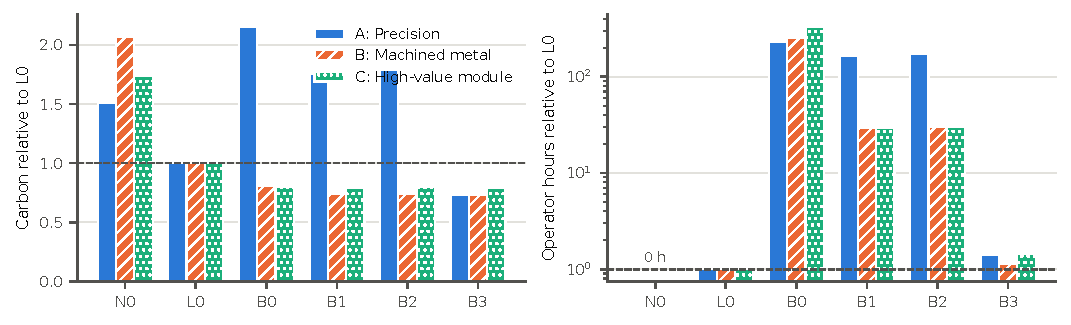
\includegraphics[width=\textwidth]{figures/fig3_regime_outcomes.pdf}
\caption{Carbon (left) and operator hours (right, logarithmic) of each regime relative to manual end-of-line inspection L0 (dashed line), at central parameter values.}
\label{fig:regimes}
\end{figure*}

\subsection{What Drives the Carbon Benefit}
The waterfall in Fig.~\ref{fig:waterfall} decomposes $\Delta C$ (B3 vs L0). Avoided field escapes contribute \PrecEscapeShare\%, \MetalEscapeShare\% and \HiValEscapeShare\%, followed by avoided unrecovered material; rework electricity is the largest negative term. Edge electricity and amortised edge hardware together amount to \PrecEdgeCarbon, \MetalEdgeCarbon{} and \HiValEdgeCarbon~\kgce{} per FU---\PrecEdgeOfBenefit\%, \MetalEdgeOfBenefit\% and \HiValEdgeOfBenefit\% of the benefit and at most \EdgeShareMax\% of B3's total footprint. In these scenarios the compute side is thus \EdgeBenefitRatioMin{} to \EdgeBenefitRatioMax{} times smaller than the benefit; even with twice the central embodied-carbon estimate of the module the edge cell stays below \HwDoubledEdgeOfBenefitMax\% of the benefit. Recall, and what an escaped defect costs, decide the outcome.

\begin{figure*}[!t]
\centering
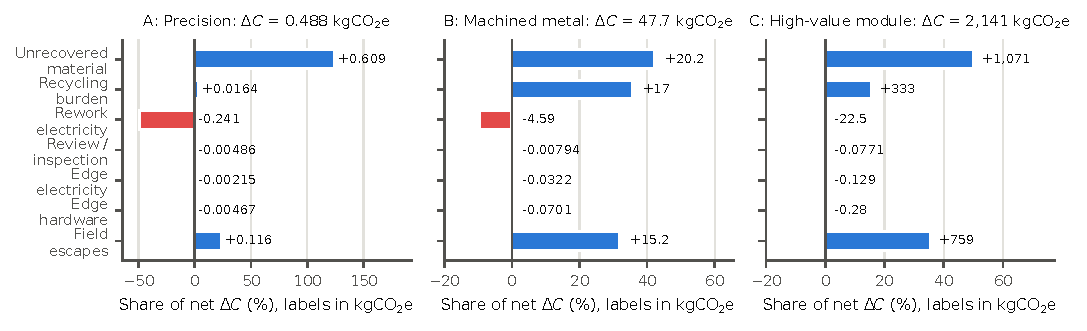
\includegraphics[width=\textwidth]{figures/fig4_carbon_waterfall.pdf}
\caption{Decomposition of $\Delta C$ (B3 vs L0) into its seven additive components, as a share of the net benefit; labels give absolute values in \kgce{} per FU. Positive values are savings.}
\label{fig:waterfall}
\end{figure*}

\subsection{Break-Even Frontiers}
\label{sec:breakeven}
Table~\ref{tab:uncertainty} and Fig.~\ref{fig:breakeven} report where $\Delta C=0$. Against no inspection, the edge cell pays back its electricity, hardware and review carbon once prevalence exceeds \PrecPiStarNZero, \MetalPiStarNZero{} and \HiValPiStarNZero~ppm. Against manual inspection, B3 stays ahead at any prevalence in scenario~A, where its advantage comes from interception timing rather than from recall, and the frontier lies at \MetalPiStarLZero{} and \HiValPiStarLZero~ppm in scenarios B and C. Holding prevalence at its central value, the edge cell could draw up to \PrecCellPowerStar, \MetalCellPowerStar{} and \HiValCellPowerStar~kW---\PrecCellHeadroom{} to \HiValCellHeadroom{} times the present value---before the benefit over manual inspection vanishes. The module's embodied carbon would have to be at least \HwStarMultLZeroMin{} times the central estimate to erase the advantage over manual inspection, and \HwStarMultNZeroMin{} times to erase that over no inspection. For scenarios B and C no break-even exists for grid intensities up to 1.5~kg/kWh, above the life-cycle intensity of coal power (median 0.82~kg/kWh~\cite{schlomer2014annex}), so no average or marginal grid factor reverses them. For the lightweight part of scenario~A the advantage over manual inspection vanishes above \PrecGammaStar~kg/kWh, about the Indian grid average and below a coal margin. The detector's recall is the decisive comparison with people. In scenarios B and C manual inspection would emit less if inspectors found more than \MetalManualRecallStar{} and \HiValManualRecallStar{} of the defects. This lies above the 70--80\% typical of visual inspection in general~\cite{see2012visual}, but human accuracy is task- and modality-dependent~\cite{aust2021comparison}, and PatchCore exceeds the higher of the two values in only \DetAboveManualStar{} of \DetCategories{} categories at q99. These break-even recalls, not the literature range, are what a line should compare with its inspectors' measured recall. In scenario~A even perfect manual recall leaves the AI regime ahead, because end-of-line discovery comes too late for rework. Net-negative regimes therefore exist---at very low defect rates, below about \PrecPiStarNZero~ppm for the lightweight part against no inspection, on carbon-intensive grids for lightweight parts, and wherever the detector's recall falls below the inspectors'.

\begin{figure}[!t]
\centering
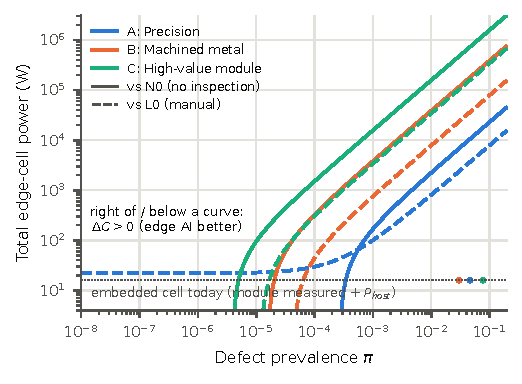
\includegraphics[width=\columnwidth]{figures/fig5_break_even_map.pdf}
\caption{Break-even frontiers $\Delta C=0$ of B3 against no inspection (solid) and manual inspection (dashed) in the plane of defect prevalence and total edge-cell power, from the bare Jetson module upward. Markers show the central scenarios with the measured module power plus the assumed $P_{host}$.}
\label{fig:breakeven}
\end{figure}

\begin{table*}[!t]
\centering
\footnotesize
\caption{Monte Carlo results (10{,}000 draws, all registry parameters) and break-even frontiers at central values. $\Delta C$ in kgCO$_2$e per 1{,}000 parts: median [5th, 95th percentile].}
\label{tab:uncertainty}
\setlength{\tabcolsep}{8pt}
\begin{tabular}{@{}lccc@{}}
\toprule
 & A: Precision & B: Machined metal & C: High-value \\
\midrule
$\Delta C$ B3 vs L0 & 0.206 [$-$0.806, 1.28] & 6.20 [$-$120, 90.1] & 317 [$-$6{,}832, 4{,}995] \\
$P(\Delta C>0)$ B3 vs L0 & 64.3\% & 54.5\% & 53.7\% \\
$P(\Delta C>0)$ B3 vs L0, correlated scores & 58.9\% & 51.8\% & 51.6\% \\
$\Delta C$ B3 vs N0 & 1.70 [0.617, 3.71] & 185 [57.9, 403] & 10{,}816 [4{,}258, 22{,}686] \\
$\Delta C$ B3 vs B0 & 3.29 [1.26, 7.71] & 16.4 [4.47, 45.3] & $-$9.56 [$-$226, 118] \\
$P(\Delta C>0)$ B3 vs B0 & 100.0\% & 99.7\% & 45.4\% \\
$P(\mathrm{SQI}_{bal}>0)$ B3 vs L0 & 37.6\% & 37.9\% & 3.6\% \\
Edge share of B3 carbon & 0.3\% & 0.071\% & 0.0038\% \\
\midrule
$\pi^\star$ vs N0 & 342 ppm & 20 ppm & 5 ppm \\
$\pi^\star$ vs L0 & none ($\Delta C>0$) & 64 ppm & 17 ppm \\
$P^\star_{cell}$ vs L0 & 3.65 kW & 23.7 kW & 265 kW \\
$r^\star_{L0}$ (manual recall) & none ($\Delta C>0$) & 94.1\% & 96\% \\
$\gamma^\star$ in [0, 1.5] & 0.719 & none ($\Delta C>0$) & none ($\Delta C>0$) \\
$C_{hw}^\star$ vs L0 (multiple of central) & 105$\times$ & 682$\times$ & 7{,}636$\times$ \\
$\delta^\star$ (relative recall loss of B3, vs B0) & none ($\Delta C>0$) & 6.11\% & 0.471\% \\
\bottomrule
\end{tabular}
\end{table*}


\subsection{Uncertainty and Global Sensitivity}
\label{sec:uncertainty}
We say a regime beats another when it emits less carbon per functional unit ($\Delta C>0$). Across \MonteCarloDraws{} draws of all \UncertainParams{} uncertain parameters, B3 beats no inspection in every draw (\PrecMcProbNZero\%, \MetalMcProbNZero\% and \HiValMcProbNZero\%) but beats manual inspection in only \PrecMcProb\%, \MetalMcProb\% and \HiValMcProb\% of draws, with median $\Delta C$ of \PrecMcMedian, \MetalMcMedian{} and \HiValMcMedian~\kgce{} (5th--95th percentiles in Table~\ref{tab:uncertainty}; Fig.~\ref{fig:uncertainty}, left). The reason is the measured spread of detector recall at the q99 threshold, from \DetRecallMin{} to \DetRecallMax{} across categories, around a median just above the manual recall. The 95th percentile of the edge share of B3's footprint is \PrecMcEdgeShareHigh\%, \MetalMcEdgeShareHigh\% and \HiValMcEdgeShareHigh\%. Fig.~\ref{fig:prcc} decomposes the variance of $\Delta C$ ($\SobolBaseRows$ base rows per Sobol matrix). The largest total-order index belongs to \PrecSobolTop{} in scenario~A ($S_T=\PrecSobolTopST$), \MetalSobolTop{} in B ($\MetalSobolTopST$) and \HiValSobolTop{} in C ($\HiValSobolTopST$). First-order effects carry most of the variance; interactions account for \SobolInteractionMin--\SobolInteractionMax\%, so the monotone PRCC ranking (top coefficients $\PrecTopPrcc$, $\MetalTopPrcc$ and $\HiValTopPrcc$) is a fair summary, and its sign gives the direction of each effect. All edge-cell parameters---edge power, host power, hardware embodied carbon and lifetime---have $S_T\le\EdgeSobolMax$ and $|\mathrm{PRCC}|\le\EdgePrccMax$. Grid intensity acts mainly through rework and review electricity, which B3 increases, so its effect on $\Delta C$ is negative and matters most in scenario~A, where little embodied carbon is at stake. Detector recall alone carries $S_T=\RecallSobolMin$--$\RecallSobolMax$: measuring the detector's recall on a line's own defects, and setting its threshold accordingly (Section~\ref{sec:thresholds}), would narrow the uncertainty far more than better compute measurements.

These indices assume independent inputs. As a stress test we imposed Spearman rank correlations of $\pm0.5$ and $\pm0.8$ on each of the \StressPairs{} pairs of \StressParams{} influential inputs in turn---detector and manual recall, prevalence, part mass, material factor, recovery fraction, recycling burden, rework energy, reworkability and the collateral multiplier---with a Gaussian copula and otherwise unchanged draws. The probability that B3 beats manual inspection moved by at most \StressShiftMax{} percentage points; the probability that it beats no inspection did not change. A positive correlation between detector and manual recall, plausible when hard-to-see defects defeat both, raised it by at most \StressRecallShiftMax{} points. The conclusions are therefore not an artefact of the independence assumption, although a line-specific joint distribution could still differ.

\begin{figure*}[!t]
\centering
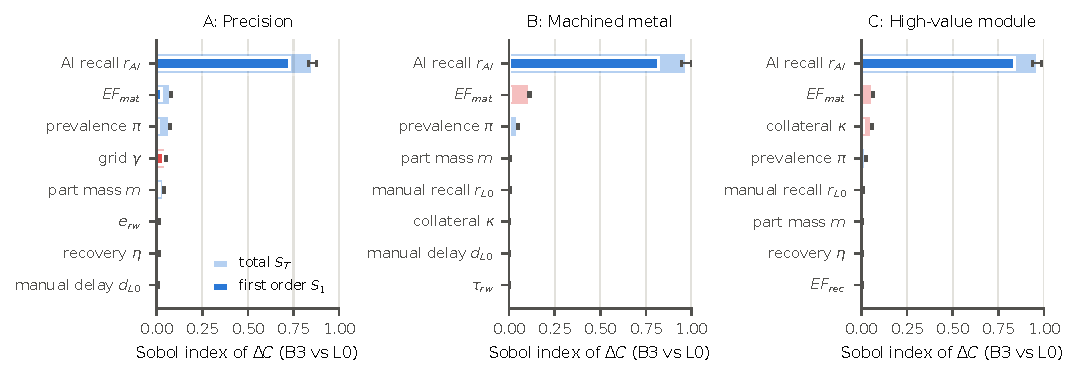
\includegraphics[width=\textwidth]{figures/fig6_global_sensitivity.pdf}
\caption{Sobol indices of $\Delta C$ (B3 vs L0) for the eight parameters with the largest total-order index per scenario: total $S_T$ (wide bars, 95\% bootstrap intervals) and first-order $S_1$ (narrow bars). Colour gives the sign of the partial rank correlation (blue: raises $\Delta C$; red: lowers it).}
\label{fig:prcc}
\end{figure*}

\subsection{Structural Sensitivity: Recycled-Content Substitution}
\label{sec:structural}
The reference model lets recovered scrap displace virgin material one-to-one. If it displaces only half ($s=0.5$) or nothing ($s=0$), scrap becomes more costly. Manual inspection scraps more defects than B3 because it finds them too late for rework, so the advantage of B3 over manual inspection grows: the share of Monte Carlo draws in which B3 emits less rises to \SubHalfProbMin--\SubHalfProbMax\% at $s=0.5$ and \SubZeroProbMin--\SubZeroProbMax\% at $s=0$. Against no inspection the saving shrinks, because intercepted defects are scrapped rather than escaping, but B3 still emits less in at least \SubZeroProbNZeroMin\% of draws at $s=0$. One-to-one substitution is therefore the conservative choice for the comparison with manual inspection.

\subsection{Alert Policy, Workload and the Recall Margin}
B0--B3 share the same edge cell, so differences among them isolate the alert policy. Smoothing alone (B1) removes most false alerts on good parts, but it raises glare alerts, and neither B1 nor persistence without the latch (B2) changes the \AlertsPerDefectMin--\AlertsPerDefectMax{} alerts each defect raises (Table~\ref{tab:policies}); their operator hours differ by at most \BOneBTwoHoursDiffMax\%. The incident latch of B3 collapses repeat alerts to one per defect. Relative to B0, B3 saves \PrecDeltaHvsBZero, \MetalDeltaHvsBZero{} and \HiValDeltaHvsBZero~operator hours and \PrecDeltaEvsBZero, \MetalDeltaEvsBZero{} and \HiValDeltaEvsBZero~kWh per FU, and $\Delta C=\PrecDeltaCvsBZero$, \MetalDeltaCvsBZero{} and \HiValDeltaCvsBZero~\kgce{}. The Monte Carlo analysis confirms the carbon saving in \PrecMcProbBZero\% and \MetalMcProbBZero\% of draws in scenarios A and B, but only in \HiValMcProbBZero\% in scenario~C, for the reason explained next. Two effects limit it. First, the persistence delay costs reworkability where it decays fast: in scenario~C it loses \HiValDelayMaterialCost~kg of material per FU relative to smoothing alone, so B1 emits \HiValBOneCarbonEdge~\kgce{} (under 0.1\%) less than B3 there; B1, however, needs \HiValReviewersBOne{} reviewers where B3 needs one. Second, any recall that persistence loses turns into field escapes. With independent scores the companion study measured no loss on sustained defects, but its \PaperAShortK-of-\PaperAShortN{} persistence filter misses short ones: the full policy catches \PaperAShortRecallOne\% of defects visible for one frame and \PaperAShortRecallEight\% of those visible for eight. The ledger therefore bounds the loss by the 8-frame value, \PersistLossMax\%, and we solve for the recall loss $\delta^\star$ at which B3's advantage over B0 vanishes (Fig.~\ref{fig:uncertainty}, right). In scenario~A no such loss exists: B0's review electricity outweighs any escapes recall could avoid. In scenarios B and C the margin is \MetalRecallLossStar\% and \HiValRecallLossStar\% of the defects single-frame thresholding flags. Combined with the measured short-defect recall, this becomes a requirement on the inspection station: a defect must stay in view for at least \MetalVisibleFrames{} frames (\MetalVisibleMs~ms) in scenario~B and \HiValVisibleFrames{} frames (\HiValVisibleMs~ms) in scenario~C for persistence to cost less recall than the margin. Where parts pass the camera faster, temporal filtering must preserve recall to within a fraction of a percent; the ledger allows up to \PersistLossMax\%, which is why B3 beats B0 in only a minority of scenario-C draws.

\begin{figure*}[!t]
\centering
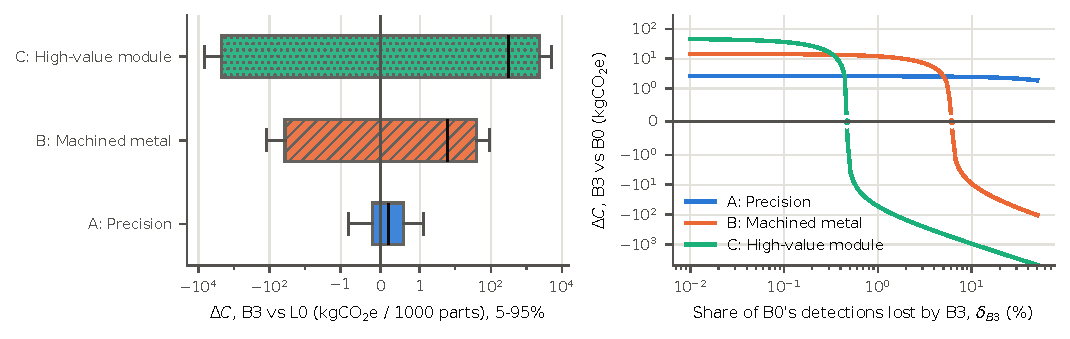
\includegraphics[width=\textwidth]{figures/fig7_uncertainty_and_tradeoff.pdf}
\caption{Left: Monte Carlo distribution of $\Delta C$ for B3 vs manual inspection (box: quartiles; whiskers: 5th--95th percentile; symmetric logarithmic axis, linear between $-1$ and 1). Right: $\Delta C$ of B3 vs single-frame thresholding B0 as a function of the share of B0's detections that B3 loses, $\delta_{B3}$; markers show the break-even $\delta^\star$.}
\label{fig:uncertainty}
\end{figure*}

\subsection{Correlated Scores, Held-Out Images, Alarm Baselines and the Cry-Wolf Risk}
\label{sec:alarms}
The companion study's main runs draw each frame's score independently, which real video does not do. When it repeated its workloads with temporally correlated scores ($\rho=0.9$ per frame), runs of good frames above threshold passed every persistence test: the full policy raised \PaperACorrFaFull{} false alerts per hour on good parts instead of none, and it missed \CorrRecallLossFull\% of the sustained defects single-frame thresholding flagged within 15 frames of onset (Table~\ref{tab:policies}). We repeat the whole analysis with these measurements (Tables~\ref{tab:alarms} and~\ref{tab:alertsets}). B3's carbon advantage over manual inspection at central values falls to \PrecCorrDeltaCvsLZero, \MetalCorrDeltaCvsLZero{} and \HiValCorrDeltaCvsLZero~\kgce{} per FU, and it beats manual inspection in \PrecCorrMcProb\%, \MetalCorrMcProb\% and \HiValCorrMcProb\% of Monte Carlo draws; against no inspection it still emits less in every draw. Its review load rises to $\rho=\CorrRhoBThreeMin$--$\CorrRhoBThreeMax$, i.e.\ \CorrReviewersBThreeMin--\CorrReviewersBThreeMax{} reviewers in every scenario. The independent-score workloads are therefore an optimistic bound on the alert burden, as the companion study notes.

The companion study also reran every workload on \PaperAVisaCategories{} held-out VisA categories with its policy and parameters frozen. VisA defects score weakly against thresholds calibrated on good parts, and persistence then delays or suppresses them: the full policy loses \VisaRecallLossFull\% of the defects single-frame thresholding flags (\VisaCorrRecallLossFull\% with correlated scores), the delay-timer \VisaRecallLossTimer\% and smoothing with hysteresis \VisaRecallLossHyst\%. With these measurements B3 saves only \PrecVisaDeltaCvsLZero~\kgce{} per FU against manual inspection in scenario~A and emits more than manual inspection in scenarios B and C ($\Delta C=\MetalVisaDeltaCvsLZero$ and $\HiValVisaDeltaCvsLZero$~\kgce{}); it beats manual inspection in \VisaMcProbLMin--\VisaMcProbLMax\% of Monte Carlo draws, and in \VisaCorrMcProbLMin--\VisaCorrMcProbLMax\% with correlated scores (Table~\ref{tab:alertsets}). It still beats no inspection in every draw. Single-frame thresholding keeps the detector's recall but needs \VisaReviewersBZeroMin--\VisaReviewersBZeroMax{} reviewers. Smoothing with hysteresis (E2), which reacts within a few frames, keeps a saving in all three scenarios (\PrecVisaETwoDeltaC, \MetalVisaETwoDeltaC{} and \HiValVisaETwoDeltaC~\kgce{} per FU) and beats manual inspection in \VisaETwoMcProbMin--\VisaETwoMcProbMax\% of draws. These runs pair the VisA alert losses with the pooled detector recall of Section~\ref{sec:detector}, so they are a stress test rather than a VisA-specific forecast. They show that the recall an alert policy preserves on weak defect scores matters as much as the false alerts it suppresses.

\begin{table*}[!t]
\centering
\footnotesize
\caption{The full policy B3 with each of the companion study's alert-measurement sets: MVTec~AD (the primary values) and the held-out VisA categories, each with independent and with temporally correlated frame scores. $\delta_{B3}$: share of the defects flagged by single-frame thresholding that B3 does not flag within 15 frames; $\rho$: single-reviewer utilization; PPV: alert precision; $\Delta C$: carbon saving against manual inspection at central values (kgCO$_2$e per 1{,}000 parts); $P$: share of Monte Carlo draws with $\Delta C>0$; $\omega^\star$: reviewer distrust at which the saving vanishes.}
\label{tab:alertsets}
\setlength{\tabcolsep}{4pt}
\begin{tabular}{@{}llrrrrrr@{}}
\toprule
Alert measurements & Scenario & $\delta_{B3}$ & $\rho$ & PPV & $\Delta C$ & $P$ & $\omega^\star$ \\
\midrule
MVTec AD, independent & A: Precision & 0.0\% & 1.43 & 77\% & 0.488 & 64.3\% & none \\
 & B: Machined metal & 0.0\% & 0.38 & 13\% & 47.7 & 54.5\% & 0.23 \\
 & C: High-value module & 0.0\% & 0.36 & 8.4\% & 2{,}141 & 53.7\% & 0.24 \\
\midrule
MVTec AD, correlated ($\rho=0.9$) & A: Precision & 2.6\% & 4.59 & 25\% & 0.415 & 58.9\% & 0.39 \\
 & B: Machined metal & 2.6\% & 3.50 & 1.4\% & 41.2 & 51.8\% & 0.18 \\
 & C: High-value module & 2.6\% & 3.49 & 0.9\% & 1{,}889 & 51.6\% & 0.20 \\
\midrule
VisA, independent & A: Precision & 22.9\% & 1.43 & 79\% & 0.157 & 32.6\% & 0.68 \\
 & B: Machined metal & 22.9\% & 0.35 & 14\% & $-$6.22 & 17.9\% & $<0$ at 0 \\
 & C: High-value module & 22.9\% & 0.33 & 9.5\% & $-$108 & 16.6\% & $<0$ at 0 \\
\midrule
VisA, correlated ($\rho=0.9$) & A: Precision & 29.4\% & 3.35 & 37\% & 0.0421 & 19.6\% & 0.07 \\
 & B: Machined metal & 29.4\% & 2.18 & 2.5\% & $-$21.8 & 8.2\% & $<0$ at 0 \\
 & C: High-value module & 29.4\% & 2.16 & 1.6\% & $-$745 & 7.7\% & $<0$ at 0 \\
\bottomrule
\end{tabular}
\end{table*}


The accounting so far also assumes that reviewers keep every truly defective part the cell diverts. Operators, however, learn how reliable alarms are and comply roughly in proportion to that reliability~\cite{bliss1995probability}, although trained controllers can remain largely compliant~\cite{wickens2009false}. In a detect-and-divert cell, non-compliance means releasing a defective part back to the line, where it escapes. We model the released share of true detections as $\omega(1-\mathrm{PPV})$, where PPV (positive predictive value, or alert precision) is the share of alerts that concern a defect, $\omega=0$ is full compliance (the value used elsewhere in this paper) and $\omega=1$ is full probability matching, and sweep $\omega$ (Fig.~\ref{fig:crywolf}). The latch that makes B3 operationally feasible also lowers its precision on slow lines: each defect now raises about one alert, while glare alerts keep arriving at a fixed rate per hour. With independent scores, B3's PPV is \PrecPpvBThree\% on the fast line of scenario~A but only \MetalPpvBThree\% and \HiValPpvBThree\% in scenarios B and C, and its advantage over manual inspection vanishes above $\omega^\star=\MetalOmegaStar$ and \HiValOmegaStar{} there, while in scenario~A it survives even full probability matching. With correlated scores, PPV falls to \PrecCorrPpvBThree\%, \MetalCorrPpvBThree\% and \HiValCorrPpvBThree\%, and $\omega^\star$ to \PrecCorrOmegaStar, \MetalCorrOmegaStar{} and \HiValCorrOmegaStar, so a modest degree of distrust erases the benefit in every scenario.

The textbook baselines trade these quantities differently (Table~\ref{tab:alarms}). Delay timers trade false alarms against missed alarms and delay~\cite{zhou2025onoff}. The delay-timer E1 and decision fusion E3, which require consecutive raw evidence, raise almost no glare alerts (\PaperAGlareTimer{} per burst against \PaperAGlareFull{} for B3), so with independent scores E1 reaches a PPV of \MetalPpvEOne\% and \HiValPpvEOne\% in scenarios B and C, against \MetalPpvBThree\% and \HiValPpvBThree\% for B3. On MVTec~AD they are charged a recall loss of \EOneRecallLoss\%, because the companion study counts a defect first flagged more than 15 frames after onset as missed. This lowers their saving to \MetalDeltaCEOne{} and \HiValDeltaCEOne~\kgce{} in scenarios B and C; if such late flags still divert the part, it is within \EOneLateGapMax\% of B3's. Smoothing with hysteresis, E2, matches B3's carbon saving with independent scores and keeps the largest saving with correlated scores (\MetalCorrDeltaCETwo{} and \HiValCorrDeltaCETwo~\kgce{} in scenarios B and C), with \CorrReviewersETwoMin--\CorrReviewersETwoMax{} reviewers. No single alarm design dominates on every criterion. Where alerts are rare and mostly glare, the release decision should not rest on the reviewer's judgement alone: diverted parts should be re-inspected before release, and glare suppression is worth more than its electricity suggests.

\begin{table*}[!t]
\centering
\footnotesize
\caption{Alarm designs at central parameter values, with Paper A's alert measurements under independent and under temporally correlated ($\rho=0.9$) frame scores: single-reviewer utilization $\rho$, alert precision (PPV), carbon saving against manual inspection $\Delta C$ (kgCO$_2$e per 1{,}000 parts, full reviewer compliance) and the reviewer distrust $\omega^\star$ at which that saving vanishes (``none'': the regime stays ahead even at $\omega=1$).}
\label{tab:alarms}
\setlength{\tabcolsep}{4pt}
\begin{tabular}{@{}llrrrrrrrr@{}}
\toprule
 & & \multicolumn{4}{c}{Independent scores} & \multicolumn{4}{c}{Correlated scores ($\rho=0.9$)} \\
\cmidrule(lr){3-6}\cmidrule(l){7-10}
Scenario & Alarm & $\rho$ & PPV & $\Delta C$ & $\omega^\star$ & $\rho$ & PPV & $\Delta C$ & $\omega^\star$ \\
\midrule
A: Precision & B3 full policy (latch) & 1.43 & 77\% & 0.488 & none & 4.59 & 25\% & 0.415 & 0.39 \\
 & E1 delay-timer & 1.38 & 93\% & 0.429 & none & 6.72 & 25\% & 0.391 & 0.37 \\
 & E2 EMA + hysteresis & 2.08 & 83\% & 0.483 & none & 4.04 & 48\% & 0.460 & 0.62 \\
 & E3 decision fusion & 1.13 & 91\% & 0.432 & none & 6.14 & 18\% & 0.398 & 0.35 \\
\midrule
B: Machined metal & B3 full policy (latch) & 0.38 & 13\% & 47.7 & 0.23 & 3.50 & 1\% & 41.2 & 0.18 \\
 & E1 delay-timer & 0.16 & 36\% & 38.0 & 0.26 & 5.10 & 1\% & 40.9 & 0.18 \\
 & E2 EMA + hysteresis & 0.43 & 18\% & 47.8 & 0.25 & 2.17 & 4\% & 47.5 & 0.21 \\
 & E3 decision fusion & 0.14 & 31\% & 38.0 & 0.24 & 5.08 & 1\% & 40.9 & 0.18 \\
\midrule
C: High-value module & B3 full policy (latch) & 0.36 & 8\% & 2{,}141 & 0.24 & 3.49 & 1\% & 1{,}889 & 0.20 \\
 & E1 delay-timer & 0.14 & 26\% & 1{,}732 & 0.25 & 5.08 & 1\% & 1{,}889 & 0.20 \\
 & E2 EMA + hysteresis & 0.40 & 12\% & 2{,}150 & 0.25 & 2.14 & 3\% & 2{,}148 & 0.22 \\
 & E3 decision fusion & 0.13 & 22\% & 1{,}732 & 0.24 & 5.06 & 1\% & 1{,}889 & 0.20 \\
\bottomrule
\end{tabular}
\end{table*}


\begin{figure*}[!t]
\centering
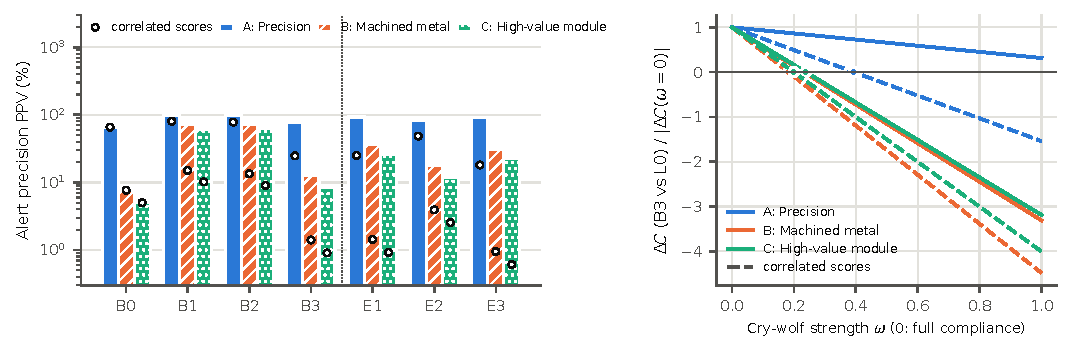
\includegraphics[width=\textwidth]{figures/fig11_cry_wolf.pdf}
\caption{Cry-wolf risk. Left: alert precision (share of alerts on defective parts, logarithmic) of each alert policy and alarm baseline with independent frame scores (bars) and correlated scores (circles). Right: benefit of B3 over manual inspection as reviewers release diverted defects in proportion to alert unreliability, $\omega(1-\mathrm{PPV})$, normalised to full compliance, for independent (solid) and correlated (dashed) scores; markers show the break-even $\omega^\star$.}
\label{fig:crywolf}
\end{figure*}

\subsection{Carbon-Optimal Detection Thresholds}
\label{sec:thresholds}
Alarm budgets such as ``at most five false alarms per 1{,}000 parts'' are set for operators, not for carbon. For a one-shot station that takes one image per part and diverts it above a threshold, each point of a measured operating curve fixes recall and false-positive rate; the accounting model then gives total carbon, including the review electricity of every false diversion. We pick the carbon-optimal point on the same measured curve on which we evaluate it, so it is an in-sample optimum and its saving an upper bound on what a threshold tuned on a line's own data can reach. Fig.~\ref{fig:detector} (right) compares it with q99 and with the alarm budget over all \OptPairs{} scenario--category pairs. With the available nominal images the budget is attainable in only \BudgetFeasible{} of the \DetCategories{} categories, where its median false-positive rate is \BudgetFprMedian\%; there the optimum is never stricter than the budget. The optimum is more permissive than q99 in \OptMorePermissive{} pairs, with a median false-positive rate of \OptFprMedian\% and up to \OptFprMax\%. Where the detector is weakest the gain is largest: for \OptWorstCategory{} (\OptWorstDataset), raising the false-positive rate to \OptFprWorst\% lifts recall from \OptRecallWorstQ{} to \OptRecallWorstOpt{} in scenario~C; across categories the optimum saves up to \PrecOptSavingMax, \MetalOptSavingMax{} and \HiValOptSavingMax~\kgce{} per FU in scenarios A, B and C. Constraining the threshold to need no more reviewers than q99 already does leaves the saving almost intact on the slower lines: the capped optimum captures \MetalOptSavingCapShare\% and \HiValOptSavingCapShare\% of the attainable saving in scenarios B and C. On the fast line of scenario~A the unconstrained optimum would need up to \PrecOptRhoMax{} reviewers, and the cap retains \PrecOptSavingCapShare\%. At the capped optimum the median recall over all pairs is \OptCapRecallMedian, against \DetRecallMedian{} at q99 and \ManualRecallCentral{} for manual inspection, so a carbon-aware threshold is also what lifts the detector above human recall. Detection thresholds should therefore be tuned against escape and scrap consequences, with the reviewer budget as a constraint rather than as the objective, and validated on held-out line data.

\begin{figure*}[!t]
\centering
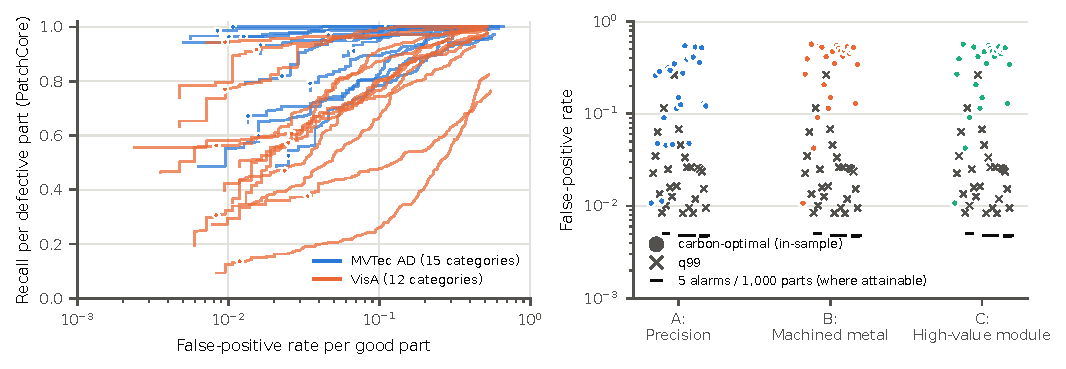
\includegraphics[width=\textwidth]{figures/fig9_detector_operating_points.pdf}
\caption{Left: measured recall versus false-positive rate per part for PatchCore on \DetMvtecCategories{} MVTec~AD (blue) and \DetVisaCategories{} VisA (orange) categories (mean over \DetSeeds{} splits; markers at q99). Right: in-sample carbon-optimal false-positive rate per category for each scenario (dots), the false-positive rate at q99 (crosses) and the rate allowed by an alarm budget of five false diversions per 1{,}000 parts in the \BudgetFeasible{} categories where it is attainable (bars).}
\label{fig:detector}
\end{figure*}

\subsection{Does More Compute Buy Recall?}
Two results above point the same way: recall decides the comparison with manual inspection, and the edge cell's electricity barely registers. Spending compute on recall should therefore pay. We tested two ways of doing so on all \DetCategories{} categories, measuring each on the Jetson in FP16 with the protocol of Section~\ref{sec:measure}: a roughly six-times larger backbone, WideResNet-50~\cite{zagoruyko2016wide} as in the original PatchCore~\cite{roth2022patchcore}, at the same $224\times224$ resolution; and the ResNet-18 at twice the resolution, $448\times448$ (Fig.~\ref{fig:compute}). The larger backbone raises recall at q99 on MVTec~AD (median \CrWrnMvtecRecall{} vs \CrPcMvtecRecall) but not on VisA (\CrWrnVisaRecall{} vs \CrPcVisaRecall), and its worst category falls to \CrWrnWorstRecall, at \CrWrnEnergyRatio{} times the energy per frame. Higher resolution helps where the base detector fails: VisA recall rises to \CrHiresVisaRecall{}, the worst category from \CrPcWorstRecall{} to \CrHiresWorstRecall, and the median over all categories from \CrPcRecall{} to \CrHiresRecall, at \CrHiresFrameMJ~mJ per frame (\CrHiresEnergyRatio{} times the base pipeline, \CrHiresActiveW~W above idle). The extra electricity and hardware share cost \PrecCrHiresExtra, \MetalCrHiresExtra{} and \HiValCrHiresExtra~\kgce{} per FU, while the mean benefit over manual inspection across categories grows by \PrecCrHiresGain, \MetalCrHiresGain{} and \HiValCrHiresGain~\kgce{}, at least \CrHiresPaybackMin{} times the extra cost. The share of categories in which B3 beats manual inspection rises from \PrecCrPcShare\%, \MetalCrPcShare\% and \HiValCrPcShare\% to \PrecCrHiresShare\%, \MetalCrHiresShare\% and \HiValCrHiresShare\%. This is one measured comparison on two benchmarks; for a given line, compute is worth spending where it buys recall on the line's own defects---here resolution for small defects---rather than on model size.

\begin{figure*}[!t]
\centering
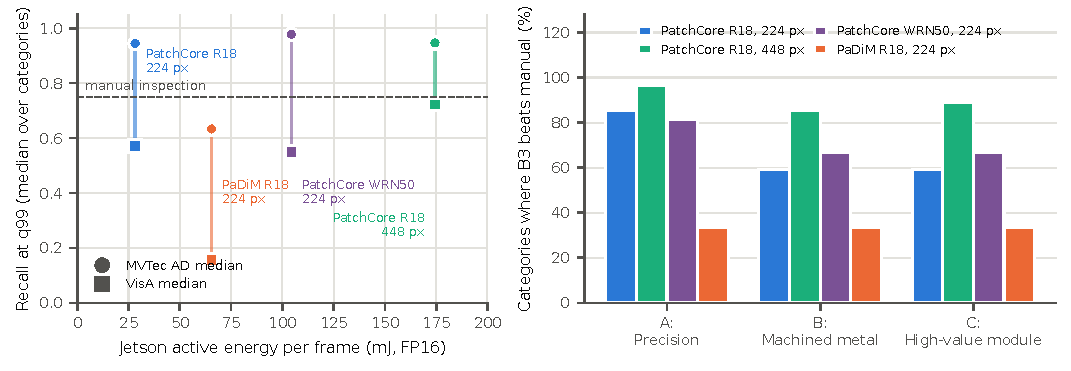
\includegraphics[width=\textwidth]{figures/fig13_compute_for_recall.pdf}
\caption{Does more compute buy recall? Left: measured Jetson energy per frame (FP16, full pipeline at 30~FPS) against median recall at q99 over the MVTec~AD (circles) and VisA (squares) categories for four detector configurations; dashed: manual inspection. Right: share of the \DetCategories{} categories in which the full policy beats manual inspection when the edge cell runs each configuration.}
\label{fig:compute}
\end{figure*}

\subsection{Generalisation: A Product Population}
To test whether the conclusions depend on the three reference scenarios, we sample \PopSize{} products: every scenario-specific parameter is drawn log-uniformly over an envelope from half the lowest to twice the highest scenario value, the defect-class mix from a Dirichlet distribution, and all other parameters from their ledger bounds. The full policy beats no inspection for \PopWinNZero\% of the products and manual inspection for \PopWinLZero\%. Products for which edge AI loses even against no inspection exist; the rule~(\ref{eq:rule}) identifies them exactly. Fig.~\ref{fig:population} (left) shows that every product lies on the side of the line $\pi=\pi^\star$ that its carbon balance predicts. The comparison with manual inspection mirrors the Monte Carlo analysis: products inherit the full measured recall range at q99, so recall again decides. Among the products that beat manual inspection, the edge cell's share of the benefit has a median of \PopEdgeShareMedian\% but exceeds 1\% for \PopEdgeShareAboveOne\% of them and reaches \PopEdgeShareNinetyFive\% at the 95th percentile (Fig.~\ref{fig:population}, right). Compute becomes relevant where the quality benefit itself is small: the products with a share above 1\% have a median benefit of \PopHighShareBenefitMedian~\kgce{} per FU against \PopLowShareBenefitMedian~\kgce{} for the others---light, low-carbon parts with few defects on slow lines. Fig.~\ref{fig:nomogram} turns the rule into a chart a practitioner can read without the model. On the embedded platform at the central grid factor, edge inspection pays back against no inspection once the product of defects per hour and embodied carbon per part exceeds about \NomogramGramsPerHour~gCO$_2$e/h; the three reference scenarios lie two to five orders of magnitude above this line, and a workstation cell or a carbon-intensive grid shifts it by less than a factor of three.

\begin{figure}[!t]
\centering
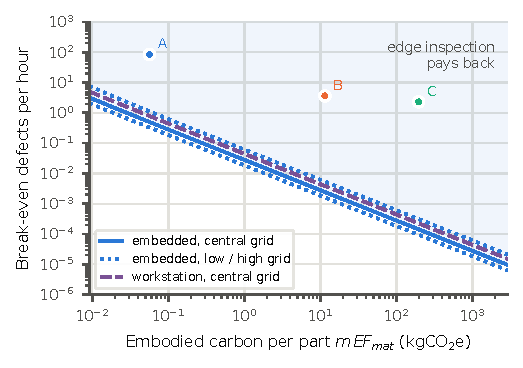
\includegraphics[width=\columnwidth]{figures/fig12_nomogram.pdf}
\caption{Break-even defect rate of the full policy against no inspection as a function of the embodied carbon per part (machined-metal parameters, rework energy proportional to mass). Edge inspection pays back above the lines. Markers: the three reference scenarios.}
\label{fig:nomogram}
\end{figure}

\begin{figure*}[!t]
\centering
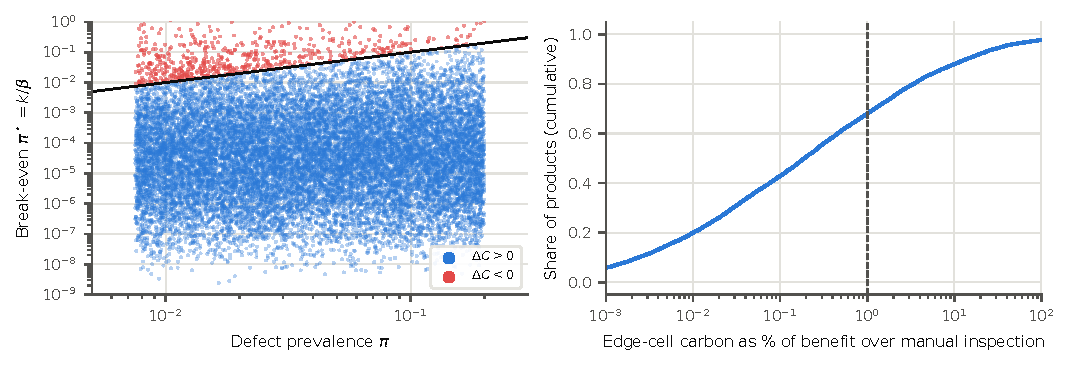
\includegraphics[width=\textwidth]{figures/fig10_decision_rule_population.pdf}
\caption{Left: \PopSize{} sampled products in the plane of defect prevalence and break-even prevalence $\pi^\star=k/\beta$; the diagonal is the decision rule~(\ref{eq:rule}): products above it ($\pi<\pi^\star$) are worse off with edge AI than without inspection, and colours show the computed sign of $\Delta C$. Right: cumulative distribution of the edge cell's carbon as a share of the full policy's benefit over manual inspection, for the products in which that benefit is positive.}
\label{fig:population}
\end{figure*}

\subsection{Multiple Criteria}
B3 improves material and carbon against manual inspection but worsens electricity ($S_E=\PrecSE$, $\MetalSE$ and $\HiValSE$) and operator time ($S_H=\PrecSH$, $\MetalSH$ and $\HiValSH$), where $S_X=(X_b-X_p)/\max(X_b,X_p)\in[-1,1]$ is a bounded relative saving, valid because all four quantities are non-negative. Any weighted index of these sub-indicators embeds value judgements: an equal-weight sum is $\PrecSqiBal$, $\MetalSqiBal$ and $\HiValSqiBal$ in the three scenarios, and it is positive for only \PrecSqiRobust\%, \MetalSqiRobust\% and \HiValSqiRobust\% of uniformly sampled weightings. We therefore report the four dimensions separately rather than as one score: stakeholders who weight electricity or operator time heavily can rank manual inspection higher even though it emits more carbon.

\section{Discussion}
\emph{Implications.} In the reference scenarios the compute footprint of edge inspection is not the decision variable. An embedded module at line rate costs \EdgeBenefitRatioMin{} to \EdgeBenefitRatioMax{} times less carbon than the benefit it enables, a workstation GPU with \FrameEnergyRatio{} times the energy per frame changes the outcome by at most \PlatformDeltaCMax\%, and, with the assumed camera and lighting allowance, the cell's peripherals draw more power than inference. Compute matters only where the quality benefit is small, for light, low-carbon parts with few defects on slow lines. Against no inspection the case for edge AI is robust in the reference scenarios and reduces to one comparison of hourly flows: the embodied carbon of the defects a line produces per hour against the roughly \NomogramGramsPerHour~gCO$_2$e/h the cell emits. Against trained inspectors there is no general answer: the decision turns on whether the detector finds more defects than the line's inspectors and finds them earlier. On curated MVTec~AD imagery PatchCore usually does; on the harder VisA imagery it often does not at a strict threshold, and the carbon benefit becomes a coin toss, more so with temporally correlated scores and less than even when the alert policy's own recall losses on VisA are included. Four design choices move the odds. Compute spent on what limits recall---here input resolution, not model size---can pay back many times over. A carbon-aware threshold accepts more false diversions in exchange for recall and, on slow lines, recovers most of the attainable saving without extra reviewers. An incident latch makes review feasible, provided persistence loses less recall than the computed margin---which it did on MVTec~AD but not on the held-out VisA images---and glare suppression keeps its alerts meaningful. Because the latch leaves glare alerts dominating on slow lines, release decisions should be backed by re-inspection rather than left to reviewers who may learn to distrust the alerts. Practitioners should therefore spend their measurement effort on recall under their own defects, on the recall of their own inspectors, on escape consequences and on alert rates---not on inference energy.

\emph{From benchmarks to production.} The comparison with manual inspection rests on detector recall measured on curated public images, a literature range for human recall and alert rates measured on simulated workloads. None of these has been observed on a production line, and benchmark-derived recall rankings may not survive distribution shift, lighting changes or a line's own defect mix~\cite{pemula2025robust}. The results should therefore be read as conditional statements about which quantities decide the outcome, not as a verdict for a given factory. The framework is built to be updated: a line that measures its detector's recall and false-positive rate on its own parts, its inspectors' recall, its alert rates on real video and its defect prevalence can replace the corresponding ledger entries and rerun the analysis unchanged.

\emph{Threats to validity.} (i) Reworkability, rework energy and manual timing remain scenario assumptions, throughput and part mass define the reference products, prevalence is proxied by scrap rates (Table~\ref{tab:parameters}), and the escape model counts only part replacement, freight and collateral damage, a lower bound that omits customer-side handling. The results are conditional on these choices; the uncertainty, break-even, structural and population analyses show how the conclusions shift. (ii) Manual recall is a literature range for visual inspection in general~\cite{see2012visual}, and human accuracy depends on the task and the inspection modality~\cite{aust2021comparison}; we therefore report the break-even manual recall that a line can compare with a measurement of its own inspectors. (iii) The alert rates come from simulated workloads in~\cite{sengar2026paperA}, with synthetic glare and sensor channels and scores sampled from small per-category pools; the glare rate and the reviewer service rate are assumptions; alerts per defect were measured on 2--8~s defect episodes and are applied unchanged regardless of how long a part stays in view. The two score models, independent and correlated, bracket the effect of temporal structure, but real inspection video may differ from both. The held-out VisA runs test the alert policies on harder images, but the accounting combines their episode-level recall losses with the detector's per-image recall from separate benchmark runs, and a defect flagged later than 15 frames counts as missed. (iv) The embedded measurement covers the whole module but not the carrier board, camera and lighting, and the workstation measurement covers the GPU only; both gaps enter through $P_{host}$, which leaves the conclusions unchanged even at its upper bound. Neither on-board sensor was checked against an external reference meter; their readings are used as reported, and the platform comparison inherits their different boundaries. The workstation GPU also served the host desktop under WSL2, and NVML sensors have documented sampling limitations~\cite{yang2024accurate}; long paced windows, repeats and robust statistics mitigate these effects without removing them. The Jetson's embodied carbon is a model estimate for the module alone~\cite{halder2025carbon,gupta2022act}. (v) Detector recall and false-positive rates come from two public benchmarks with few nominal test images per category, measured on single images; production imagery, distribution shift~\cite{pemula2025robust}, drift and multi-view stations change them, and benchmark rankings may not transfer to a given line. This is why we report recall over all \DetCategories{} categories rather than a single value, and why the conclusions against manual inspection are stated conditionally on recall. The carbon-optimal thresholds are in-sample optima. Multi-camera cells or higher frame rates scale $E_{edge}$ proportionally; even a 100-fold increase stays below the frontiers of Fig.~\ref{fig:breakeven}. (vi) Reworkability decay, the detect-and-divert architecture, the single-reviewer queue and the replacement-based escape model are simplifications, and rebound effects and end-of-life treatment lie outside the boundary. (vii) The main analysis samples parameters independently; the stress test bounds the effect of pairwise rank correlations but not of every joint distribution, and Sobol indices are reported for independent inputs only~\cite{kim2025global,iooss2019shapley}.

\section{Conclusion}
With measured inputs---the power of a real PatchCore pipeline on an embedded module and on a workstation GPU, the recall of four detector configurations on \DetCategories{} categories of two public benchmarks, and alert rates of four alert policies and three alarm baselines on two benchmarks under independent and correlated frame scores---the sustainability of edge AI inspection is decided by quality, not by compute, except for products whose quality benefit is itself small. In the reference scenarios the edge cell accounts for at most \EdgeOfBenefitMax\% of the benefit, and against no inspection edge AI pays back whenever $\pi\beta>k$, which held for \PopWinNZero\% of \PopSize{} sampled products. Against manual inspection the answer is line-specific: it pays back only when the detector out-recalls the line's inspectors, which at a strict threshold holds in \McProbLMin--\McProbLMax\% of Monte Carlo draws with the MVTec~AD alert measurements, \CorrMcProbLMin--\CorrMcProbLMax\% with correlated frame scores and only \VisaMcProbLMin--\VisaMcProbLMax\% with the held-out VisA measurements, where persistence filtering loses recall; detector recall explains most of the uncertainty. Spending compute on recall, carbon-aware thresholds, an alarm design that suppresses glare without losing weak or short defects, and re-inspection of released parts can turn this coin toss into a reliable benefit, but production-grounded measurements of recall, alert rates and inspector performance on the same line are what would settle it.


% Shared by main.tex (arXiv) and access.tex (IEEE Access). Every number is a macro from paper_b_generated_metrics.tex.
\appendices
\section{Reproducibility Checklist}
\label{app:repro}
Table~\ref{tab:repro} lists the meters, boundaries, software versions, datasets and seeds behind every result. Versions, seeds and protocol settings are written by the pipeline from the committed run metadata and scripts; the split fractions and sampling rate are constants of the committed code, and the checksum identifies the dataset archive used.

\begin{table}[!t]
\centering
\scriptsize
\caption{Reproducibility checklist.}
\label{tab:repro}
\setlength{\tabcolsep}{3pt}
\begin{tabular}{@{}l>{\raggedright\arraybackslash}p{0.66\columnwidth}@{}}
\toprule
Item & Value \\
\midrule
Embedded meter & INA3221 VDD\_IN (whole \JetsonModel{} module), 20~Hz, trapezoid-integrated over \BenchWindow~s windows \\
Embedded boundary & module only; carrier board, camera and lighting via $P_{host}$ \\
Embedded software & \JetsonLft{} (Linux \JetsonKernel), TensorRT \JetsonTensorRT, \JetsonPowerMode{} mode, Python \JetsonPython \\
Workstation meter & NVML power sensor, 20~Hz (cumulative energy counter logged, not used) \\
Workstation boundary & GPU only; host computer, camera and lighting via $P_{host}$ \\
Workstation software & \GpuName{}, driver \GpuDriver, PyTorch \TorchVersion, CUDA \CudaRuntime, Python \WsPython, WSL2 \\
Protocol & \BenchFps~FPS paced, \BenchRepeats{} repeats, 15~s idle per repeat, shuffled stage order (seed \SeedEnergy), median [min, max] \\
Units & power W; energy J/frame, kWh/FU; carbon \kgce{}/FU; FU = 1{,}000 parts \\
Datasets & MVTec~AD (official archive, MD5 \texttt{eefca59f2cede9c3fc5b6befbfec275e}); VisA (official 1-class split); scores only redistributed \\
Detector splits & 60/20/20 fit/calibration/held-out, seeds \DetSeedList \\
Alert measurements & companion study~\cite{sengar2026paperA}, revision \texttt{\PaperACommit}, recomputed and checked against its printed values \\
Uncertainty & \MonteCarloDraws{} triangular draws (seed \SeedMonteCarlo); Sobol \SobolBaseRows{} base rows (seed \SeedMonteCarlo); population \PopSize{} products (seed \SeedPopulation) \\
Verification & SymPy proofs, dimensional checks and paper-vs-code evaluation of every equation; claim checks and drift test in continuous integration \\
\bottomrule
\end{tabular}
\end{table}

\section*{Data and Code Availability}
Code, the parameter ledger, raw power traces, detector scores, the Paper A snapshot, all processed results, and the scripts that generate every figure, table and number are available at \url{https://github.com/sengarutk/sustainable-edge-quality-intelligence} (MIT license); the imported alert measurements are pinned to revision \texttt{\PaperACommit} of \url{https://github.com/sengarutk/edge-quality-intelligence}. Images of the public datasets are not redistributed.

\section*{Acknowledgment}
The author used an AI assistant, Claude (Anthropic, model Claude Opus 5.5), in preparing this work: to develop and test parts of the analysis and measurement code, to draft and revise text in all sections, to check consistency between the code, the results and the manuscript, and to search for references and check them against Crossref. All measurements were made on the author's own hardware, every reported number is generated by the released pipeline from committed data, and the author reviewed and verified all AI-assisted content and takes full responsibility for this paper.


\bibliographystyle{IEEEtran}
\bibliography{references}

\begin{IEEEbiographynophoto}{Utkarsh Sengar}
is pursuing the B.Tech.\ degree in computer science and engineering at the Indian Institute of Technology Dharwad, Dharwad, India. Research interests include edge artificial intelligence for industrial visual inspection, alarm management for anomaly detectors, and the energy and carbon accounting of computing systems.
\end{IEEEbiographynophoto}

\EOD

\end{document}
